\documentclass[12pt,a4paper,spanish]{book}

\usepackage{babel}
\usepackage[latin1]{inputenc}
\usepackage{graphicx}
\usepackage{hyperref}
\hyphenation{nues-tros modi-ficar determi-nista diferen-tes ha-biendo cons-truir se-leccionamos pro-ducciones conside-ramos corres-pondiente do-cumento ele-vado pro-blema admi-nistrador Automa-taP vi-sualizamos TALFi docu-mentaci
repre-sentaci ante-riormente vi-sualizaci mini-mizaci corres-ponden des-cubrimos gene-ran 
ti-caIC ma-nera si-mulaci he-rramientas deter-minista re-chazadas go-bierna re-presenta Re-presentamos rea-lizar acce-so
Mac-OS almace-namos}

%\oddsidemargin -1.0cm
\headsep 2cm
%\textwidth=16cm
%\textheight=20cm
%\parskip=4mm
%\headheight=2cm
\newcommand{\clearemptydoublepage}{\newpage{\pagestyle{empty}
\cleardoublepage}}


\begin{document}
\title{\huge{\bf{TALFi 2.0}}\\
\begin{center}

\includegraphics{escudo.jpg}
\end{center}}

\author{
Roc\'io Barrig\"{u}ete \\
Mario Huete \\
Luis San Juan \\
\\
Director: Alberto de la Encina \\
\\
}

\date{\em{Facultad de Inform\'atica \\ 
Universidad Complutense de Madrid \\ 
Curso 2009-2010 \\
Junio 2010 \\}}


% Generamos titulo e indice de contenidos
\maketitle
\newpage
\begin{center}

\includegraphics[scale=0.4]{escudo.jpg}\\
\end{center}

Se autoriza a la Universidad Complutense de Madrid a difundir y utilizar con fines acad\'emicos, no comerciales y mencionando expresamente a sus autores abajo firmantes, tanto la propia memoria, como el c\'odigo, la documentaci\'on y / o el prototipo desarrollado.\\
\newline
\newline
Fdo.:\\
\newline
Luis San Juan Germ\'an:\\
\newline
\newline
\newline
\newline
Mario Jose Huete Jim\'enez:\\
\newline
\newline
\newline
\newline
Rocio Barrig\"{u}ete Ib\'a\~nez:\\
\tableofcontents


%%%%%%%%%%%%%%%%%%%%CAPITULO 1%%%%%%%%%%%%%%%%%%%%%%%%%%
\chapter{Resumen}
TALFi naci\'o en el curso acad\'emico 2008-2009 como una aplicaci\'on de apoyo y consulta sobre teor\'ia de aut\'omatas y lenguajes formales.
Su primera versi\'on conten\'ia funcionalidad acerca de aut\'omatas finitos (deterministas, no deterministas y con transiciones vac\'ias), y expresiones regulares, as\'i como su equivalencia, simplificaci\'on y dem\'as aspectos relacionados.
Para TALFi 2.0 se han creado muchas m\'as caracter\'isticas adicionales, as\'i como la mejora de ciertos aspectos de la primera versi\'on, que no resultaban del todo intuitivos para el usuario y claros en la comprensi\'on.\\
Como nueva funcionalidad podemos encontrar el tratamiento de aut\'omatas de pila, m\'aquinas de Turing y gram\'aticas independientes de contexto. Para ello, se han a\~nadido componentes gr\'aficos para poder manipular la representaci\'on de dichos aut\'omatas, as\'i como nuevas implementaciones para definir sus comportamientos, sus transiciones m\'as complejas, as\'i como m\'etodos para minimizar, conocer equivalencias o pertenencia de palabras.\\
En cuanto a las mejoras, se mejorado la minimizaci\'on de aut\'omatas finitos, ya que detectamos fallos al aplicarlo y adem\'as hemos profundizado en los pasos que se siguen en este algoritmo, explic\'andolos de forma m\'as detallada. Por otra parte se ha diferenciado entre la apertura de un ejercicio. Esto ya lo hac\'ia la antigua versi\'on de TALFi, pero cab\'ia la posibilidad de abrir un ejercicio como un ejemplo y poder ver su soluci\'on (opci\'on no recomendable para el aprendizaje).
Con esta nueva ampliaci\'on, TALFi se convierte en una herramienta de gran expresividad dentro del entorno de los aut\'omatas y la generaci\'on de lenguajes, a la altura de otras tecnolog\'ias ya conocidas como JFLAP, etc. 


\clearemptydoublepage
%%%%%%%%%%%%%%%%%%%%CAPITULO 2%%%%%%%%%%%%%%%%%%%%%%%%%%
\chapter{Objetivos}
En esta segunda versi\'on de TALFi, como se ha mencionado antes, se ha buscado la ampliaci\'on de la herramienta inicial a\~nadi\'endole funcionalidad extra para el tratamiento de gram\'aticas independientes de contexto (GIC), aut\'omatas de pila (AP) y m\'aquinas de Turing (MT), parte muy importante de la teor\'ia de aut\'omatas y lenguajes formales, as\'i como ciertos algoritmos necesarios para su simplificaci\'on, correcci\'on y tratamiento:
\begin{itemize}
\item La inclusi\'on de aut\'omatas de pila y m\'aquinas de Turing requiri\'o nuevas clases para implementar su comportamiento, as\'i como nuevos elementos gr\'aficos para su tratamiento por parte del usuario (botones para introducir la cinta de una m\'aquina de Turing, nuevos ejemplos de las nuevas representaciones \ldots).
\item Posteriormente fue necesario diferenciar en cierta manera un aut\'omata de pila de un aut\'omata de pila determinista. Aunque TALFi no ofrece la posibilidad al usuario de decidir si el aut\'omata de pila que introduce es o no determinista, internamente TALFi si distingue este caso, ya que es una caracter\'istica importante de estos aut\'omatas dado que por naturaleza son no deterministas.
\item De forma secundaria y sin formar parte de los objetivos, tuvieron que incluirse gram\'aticas independientes de contexto, en sus formas normales de Chomsky y Greibach.
Esto era necesario porque, parte muy importante de TALFi (el algoritmo de reconocimiento de una palabra por un aut\'omata de pila) requer\'ia poder pasar de gram\'atica a aut\'omata de pila y viceversa.

\item Como parte importante de los objetivos, podemos mencionar las mejoras y arreglos realizados en TALFi 1.0:
\begin{itemize}
\item Minimizaci\'on: la minimizaci\'on en TALFi 1.0 tuvo que ser corregida, s\'olo se pod\'ia aplicar a aquellos aut\'omatas que fueran finitos y deterministas. Gracias a TALFi 2.0 la minimizaci\'on es posible adem\'as para aut\'omatas finitos no deterministas y aut\'omatas finitos no deterministas con transiciones vac\'ias, gracias al previo paso de transformaci\'on de estos dos \'ultimos tipos de aut\'omatas en un aut\'omata finito determinista.
Para cerrar de manera final la minimizaci\'on se imprime en un archivo HTML de forma detallada las tablas que se generan en este algoritmo para que quedasen m\'as claros los pasos que se van realizando.
\item TALFi 1.0 diferenciaba entre ejercicios y ejemplos, pero era posible ver la soluci\'on de un ejercicio propuesto por el profesor, si lo abr\'iamos como ejemplo. Este comportamiento no nos pareci\'o muy adecuado debido al car\'acter docente y de aprendizaje de TALFi. Dicho comportamiento fue subsanado, adem\'as de incluir mayor n\'umero de ejemplos y ejercicios.
\item Inclusi\'on de un modo \LaTeX{} con el que podemos obtener en dicho formato, tanto los aut\'omatas que se creen en TALFi, como los ejemplos, as\'i como la simplificaci\'on de las gram\'aticas anteriormente mencionadas.\\
\end{itemize}
\item Como posible mejora futura, proponemos incluir TALFi 2.0 como una aplicaci\'on web dentro de un entorno como, por ejemplo, el \htmladdnormallink{Campus Virtual UCM}{https://www.ucm.es/campusvirtual/CVUCM/index.php}. Evidentemente la herramienta segur\'ia teniendo las mismas aplicaciones, pero la identificaci\'on de usuario ya no ser\'ia necesaria dentro de la aplicaci\'on: estar\'ia ligada al tipo de login que se realizase en la web.
No ser\'ia la \'unica adaptaci\'on necesaria, pues el env\'io de ejercicios propuestos tambi\'en requiere hacer uso de los medios de comunicaci\'on con tutor del Campus Virtual UCM, para poder hacer llegar al administrador de la aplicaci\'on la soluci\'on realizada por el alumno y terminar la correcci\'on.
En TALFi 1.0 ya se diferenci\'o los tipos de usuarios que tendr\'ia la aplicaci\'on, simulando el comportamiento y garantizando su eficiencia.
\end{itemize}

\clearemptydoublepage
%%%%%%%%%%%%%%%%%%%%CAPITULO 3%%%%%%%%%%%%%%%%%%%%%%%%%%
\chapter{Informaci\'on}
\section{Antecedentes}
Existen muchas y diversas aplicaciones que operan con aut\'omatas de manera similar a como lo hace TALFi, pero la mayor\'ia de estas est\'an enfocadas a un tipo de problema en concreto.
Algunas tratan aut\'omatas finitos, otras se centran en operaciones de traducci\'on de lenguajes, algunas incorporan simulaci\'on de m\'aquinas de Turing, pero ninguna cuenta con la expresividad y riqueza de TALFi 2.0.
Para m\'as detalle de estas aplicaciones conviene visitar los siguientes enlaces:
\newline

\begin{itemize}
\item{ \noindent\url{http://www.versiontracker.com/dyn/moreinfo/win/35508} \\}
Crea y simula aut\'omatas finitos y m\'aquinas de Turing, permite guardar la informaci\'on en archivo, y abrir varios de estos archivos a la vez.
\end{itemize}
\begin{itemize}
\item{ \url{http://www.cs.duke.edu/csed/jflap/} \\}
Quiz\'a el programa m\'as conocido, puesto que se usa en la asignatura de TALF. Permite crear aut\'omatas finitos, expresiones regulares, algoritmos de conversi\'on entre aut\'omatas finitos y a expresi\'on regular, aut\'omatas de pila, gram\'aticas independientes de contexto y simulaci\'on de m\'aquinas de Turing.
\end{itemize}
\begin{itemize}
\item{ \url{http://www.ucse.edu.ar/fma/sepa/} \\}
Es espa\~{n}ol. Permite dise\~{n}ar, desarrollar y evaluar un conjunto de herramientas de software que ayude al personal docente en la ense\~{n}anza de las teor\'ias y tecnolog\'ias involucradas en los procesos de dise\~{n}o y construcci\'on de traductores de lenguajes formales.
\end{itemize}
\begin{itemize}
\item{ \url{http://www.brics.dk/automaton/} \\}
Trata aut\'omatas finitos, expresiones regulares, y operaciones de cierre sobre lenguajes regulares.
\end{itemize}


Todas estas versiones pueden ser descargadas gratuitamente.
Obviamente, como antecedente m\'as directo contamos con la primera versi\'on de TALFi.
A diferencia de los programas anteriormente mencionados, TALFi dispone de la posibilidad de ver paso a paso como se simplifica una gram\'atica, saber si una palabra puede ser reconocida por un aut\'omata de pila, generaci\'on de palabras que son reconocidas por un lenguaje y multitud de posibilidades que TALFi contempla a diferencia de sus antecesores.\\
Adem\'as, resaltar que los programas que trabajan con teor\'ia de aut\'omatas y lenguajes formales est\'an m\'as enfocados al estudiante que a los profesores que imparten esta ense\~{n}anza, y ninguno de los mencionados est\'a concebido para ser utilizado como una herramienta de comunicaci\'on y evaluaci\'on. Es el rasgo principal de TALFi, que diferencia dos perfiles de usuario, y m\'as que un apoyo en el estudio se enfoca a un posible uso real al impartir una asignatura. Y por \'ultimo lo que es \'unico en talfi es la salida que genera en HTML de los algoritmos aplicados, y por supuesto no tienen la opci\'on de generar c\'odigo en \LaTeX{}.

\section{Problemas encontrados y resueltos en\\
TALFi}
En un primer momento, tuvimos que dedicar mucho tiempo a entender el funcionamiento de la aplicaci\'on, y por tanto el c\'odigo creado por nuestros compa\~neros el a\~no pasado. A continuaci\'on describimos en que partes encontramos dificultades.

\subsection{Minimizaci\'on}

Mientras nos dedic\'abamos a ir un paso m\'as all\'a con la minizaci\'on, descubrimos varios fallos en este algoritmo, teni\'endolo que rehacer en parte, para poder cuadrarlo con los cambios que se nos hab\'ian pedido.

En primer lugar, introducimos un estado trampa llamado ``tramposo'', para aclarar el estado a d\'onde llegan las transiciones que no est\'an definidas ni tienen una arista equivalente en aut\'omatas finitos no deterministas y aut\'omatas finitos con transiciones vac\'ias.

En segundo lugar, ampliamos la informaci\'on que aparece en las casillas de la tabla que se construye para comprobar que estados son colapsables en el algoritmo de minimizaci\'on. Anteriormente, dentro de las celdas pod\'iamos encontrar:

\begin{itemize}

\item Una ``X'' si los estados no se colapsaban.

\item Un ``+'' si los estados son colapsables.

\end{itemize}

Ahora, ampliando la informaci\'on de la siguiente manera:

\begin{itemize}

\item Si los estados no son colapsables, damos los m\'otivos de por qu\'e: uno puede pertenecer a los estados finales y el otro no, o si es causado por otros dos estados que se sabe que no son colapsables y tienen tambi\'en su casilla marcada. Adem\'as, como la tabla la revisamos hasta que no hayamos marcado ninguna nueva casilla, incluimos en que n\'umero de vuelta hemos realizado el cambio en la celda.

\item Si los estados son colapsables dejamos la casilla en blanco.

\end{itemize}

V\'ease un ejemplo de la ejecuci\'on actual de la minimizaci\'on de dos aut\'omatas finitos sobre uno de los ejemplos que el a\~no pasado se usaba para mostrar el funcionamiento de este algoritmo:

Aqu\'i tenemos el aut\'omata sobre el que vamos a aplicar la minimizaci\'on, concretamente el ejemplo 7 de los aut\'omatas finitos no deterministas:\\
\begin{center}
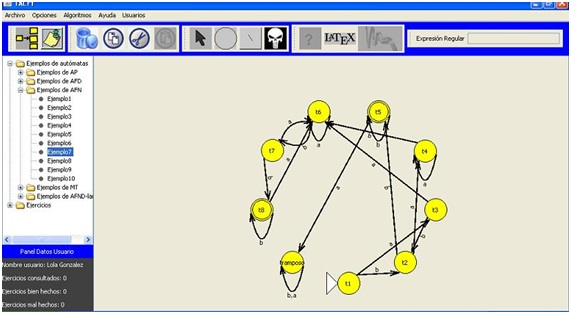
\includegraphics[width=\textwidth]{auto1.jpg}\newline \newline \newline \newline \newline 

\end{center}


Y la tabla que obtenemos en el HTML generado cuando queremos ver todos los pasos que hemos seguido en la minimizaci\'on, es la siguiente:
\newline 
\begin{center}
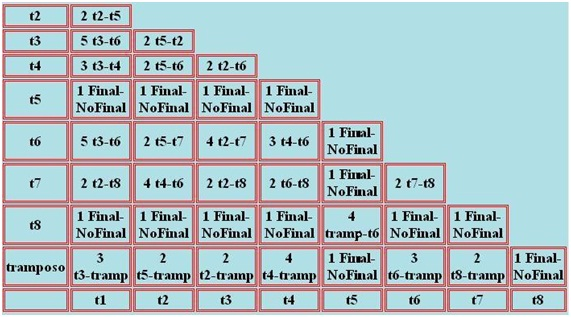
\includegraphics[width=\textwidth]{tabla1.jpg}\\
\end{center}


En cada celda podemos ver:
\begin{enumerate}
\item Si el estado de la columna es final y el de la fila no final, o viceversa, los dos estados no podr\'an colapsarse, y lo indicamos con Final-No final.
\item A partir de las casillas marcadas con estados que nunca podr\'an colapsarse, procedemos a comprobar que ocurre con el resto de casillas. Para terminar la explicaci\'on de por qu\'e se marca esa casilla, debajo o al lado indicamos que par de estados son los causantes.
\end{enumerate}

Si los estados pudieran colapsarse, la casilla no tendr\'a nada escrito dentro de ella.\\

Aqu\'i podemos ver qu\'e salida HTML se generaba para un ejemplo sencillo, el ejemplo 6 de aut\'omatas finitos deterministas en TALFi 1.0.\\ \newline \newline \newline \newline \newline \newline
Aut\'omata sobre el que aplicamos el algoritmo de minimizaci\'on:
\begin{center}
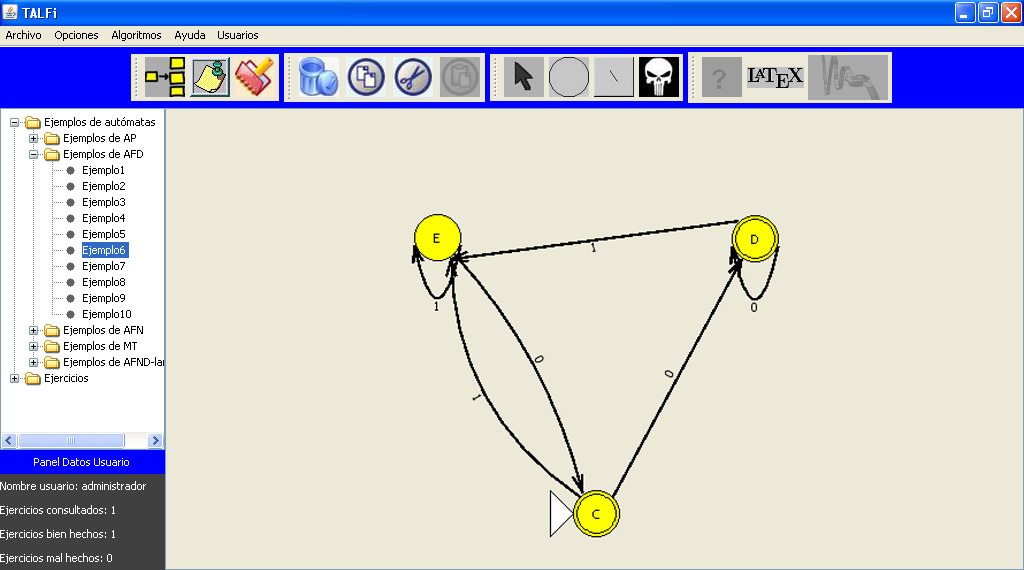
\includegraphics[width=\textwidth]{autminiantigua.jpg}\\
\end{center}

Y la tabla que se generaba era la siguiente:
\begin{center}

\includegraphics{pasosminiantigua.jpg}
\end{center}

\subsection{Intento de reconocimiento de palabras simulando la ejecuci\'on de un aut\'omata de pila\\}
Al tener la aplicaci\'on un enfoque did\'actico, la primera idea que nos vino a la cabeza para saber si una palabra es reconocida por un aut\'omata de pila, fue seguir la misma metodolog\'ia que vimos en clase de TALF. No traduc\'iamos el aut\'omata de pila en una gram\'atica, sino que \'ibamos simulando el comportamiento que ten\'ia el aut\'omata seg\'un le\'ia los s\'imbolos de una cadena.\\

B\'asicamente la idea de funcionamiento de este algoritmo es muy sencilla: Es un algoritmo recursivo, que posee backtracking, pues en muchos casos tenemos m\'as de un camino posible a seguir al procesar una cadena. Si en alg\'un momento, al terminar de consumir los s\'imbolos de la cadena, llegaba a un estado de aceptaci\'on, o se vaciaba la pila, se devolv\'ia un booleano que indicaba que la palabra era aceptada y se terminaba la ejecuci\'on del algoritmo. En caso contrario, la palabra no se aceptaba y se devolv\'ia falso.
El procedimiento que conten\'ia este algoritmo recibe como par\'ametros:
\begin{enumerate}
\item Lista de estados posibles a los que podemos ir. Tiene prioridad si existe una transici\'on que no consume s\'imbolos. La idea es la siguiente: cuando vamos a procesar el primer s\'imbolo de la cadena, con transiciones vac\'ias es trivial, porque no hemos consumido a\'un ning\'un s\'imbolo, pero si no las hubiera, recopilar\'iamos todos los posibles estados destino, y asumir\'iamos que ya hemos consumido un s\'imbolo de la cadena a reconocer.
\item Pila actual: El estado de la pila hasta el momento. En cada estado al que nos movemos va cambiando, as\'i que solo la modificamos si volvemos a llamar al procedimiento. Si en alg\'un momento se vac\'ia, y si estamos comprobando si la palabra es reconocida por estado, abortamos el procesamiento.
\item N\'umero de elementos que tiene la pila: Inclu\'ido por si en alg\'un momento sirve para detectar los ciclos de los que hemos hablado anteriormente.
\item Cima de la pila en el momento actual: Por comodidad, y por si se quiere comprobar el caso extremo de que si se ha desapilado el s\'imbolo de fondo de pila, y solo queda un s\'imbolo en la pila, pero no coinciden, se pare la simulaci\'on por no poder averiguar, si se ha terminado de vaciar la pila o no. Aqu\'i ser\'ia f\'acil averiguarlo, pero en la teor\'ia de aut\'omatas se restringe de esta manera.

\item Palabra a procesar: Se podr\'ia haber pasado s\'olo como par\'ametro el s\'imbolo actual que se procesa, pero para posibles explicaciones se incluy\'o la palabra completa.
\item \'Indice del s\'imbolo procesado: Se incluye para poder ubicar por que s\'imbolo de la cadena va la ejecuci\'on.
\item Estado: Estado actual en el que estamos, que nos sirve para poder calcular los posibles movimientos que podemos hacer.
\end{enumerate}


Este procedimiento se apoya en otros dos, que se intuyen seg\'un se ha explicado c\'omo funciona: el primero, que calcula como quedar\'a la pila para la siguiente llamada al procedimiento, y el segundo, que devuelve la lista de posibles estados a los que podemos seguir procesando con un s\'imbolo o no, si es que la transici\'on es vac\'ia, el estado actual, y la cima de pila actual.\\

Nos dimos cuenta que el algoritmo no terminaba si inclu\'iamos ciclos de transiciones vac\'ias en los que la pila no se modificase o sufriera modificaciones que no acercaban la ejecuci\'on a su final. Esto se puede arreglar de dos maneras:

\begin{itemize}

\item Dando prioridad a las aristas que consuman s\'imbolos, pues si alguna sale de alguno de los estados que componen el ciclo tendremos la oportunidad de seguir el c\'omputo por otro camino, esperando que llegue a su fin. En algunos casos es una soluci\'on valida, pero no es suficiente pues podr\'ia no llevarnos a un estado que estuviera fuera de los estados que componen el ciclo, y seguir\'iamos teniendo el mismo problema.

\item Fijando una cota que s\'olo utilizaremos en los casos en que simulando la ejecuci\'on del aut\'omata hayamos elegido seguir el camino marcado por una arista que no consuma s\'imbolos. Si entramos en un ciclo como los ya descritos, comenzamos a acumular las veces que ejecutamos el algoritmo. Si ejecutamos {\it (n\'umero de estados * n\'umero de aristas)} movimientos y no hemos avanzado en nuestro procesamiento de la cadena, asumimos que el algoritmo no terminar\'a forzando as\'i que finalize la ejecuci\'on.\\

\end{itemize}


El algoritmo se basa en dos m\'etodos: uno que indica si se reconoce o no una cierta cadena por estado final, y otro que realiza la misma acci\'on pero vaciando la pila. Los dividimos por un lado para mejorar la eficiencia, ya que se puede dar el caso de que el aut\'omata de pila no tenga ning\'un estado final, o ninguna arista desapile el s\'imbolo de fondo de pila, y devolver m\'as informaci\'on que \'unicamente concretar si la palabra es aceptada o no, dando a conocer al usuario por cu\'al de los dos m\'etodos reconoce una cadena el aut\'omata de pila. \\

\begin{itemize}

\item M\'etodo reconocedor de palabras por estado final: Se comprobar\'a que la cadena, que puede ser o si es $\epsilon$ o una cadena formada por uno o m\'as s\'imbolos del alfabeto de entrada es reconocida si hemos llegado a un estado a partir del cual no podemos ir a ning\'un otro comprobando la longitud de la cadena la cadena a reconocer, o en cambio si tiene transiciones posibles donde moverse pero hemos alcanzado el final de la cadena. En cualquier otro caso, se contin\'ua con la simulaci\'on.

\item M\'etodo reconocedor de palabras por pila vac\'ia: Se comprobar\'a si cuando llegamos a un estado donde ya no podemos movernos m\'as la pila est\'a vac\'ia o no, y si hemos alcanzado la longitud de la cadena, que podr\'a ser tambi\'en $\epsilon$ o una cadena formada por uno o m\'as s\'imbolos del alfabeto de entrada . De forma id\'entica al m\'etodo reconocedor por estado final, si no estamos en ese caso, comprobamos c\'omo se quedar\'ia la pila para el siguiente paso a realizar, y si es vac\'ia revisamos la longitud de la cadena. En caso contrario la ejecuci\'on sigue su curso.

\end{itemize}

Quiz\'a en un futuro sean pautas que alguien pueda seguir para explicar el funcionamiento de los aut\'omatas de pila. Nosotros \'ibamos a utilizarlo para probar que una palabra pertenec\'ia al lenguaje de un aut\'omata de pila, pero el coste se disparaba a exponencial, volvi\'endose intratable. Optamos por el algoritmo llamado CYK, cuyo coste es mucho mejor, ya que es c\'ubico sobre la longitud de la cadena.

\section{Introducci\'on a la ampliaci\'on de la aplicaci\'on}


TALFi 1.0 es capaz de crear aut\'omatas finitos deterministas, no deterministas, con transiciones vac\'ias y expresiones regulares.
Como algoritmos importantes cuenta con:
\begin{itemize}
\item Transformaci\'on de un aut\'omata con transiciones vac\'ias a uno no determinista.
\item Transformaci\'on de un aut\'omata no determinista a uno determinista.
\item Transformaci\'on de aut\'omata finito determinista a expresi\'on regular.
\item Minimizaci\'on de aut\'omatas finitos no deterministas.\\
\end{itemize}
La interfaz de usuario de TALFi 1.0 cuenta con un \'arbol desplegable donde podemos encontrar ejemplos y ejercicios que la primera versi\'on de TALFi es capaz de llevar a cabo. Tambi\'en dispone de los usuales controles para modificar, copiar, pegar, borrar cualquier aspecto de la figura que creemos en la zona central de la interfaz.

TALFi 2.0 respeta esta estructura y le a\~nade una colecci\'on de ejemplos de ejercicios de aut\'omatas de pila y m\'aquinas de Turing. Sobre los primeros, podremos realizar un estudio a fondo del lenguaje independiente de contexto que generan, obteniendo los siguientes resultados:
\begin{itemize}
\item Lista de palabras aleatorias que pertenecen al lenguaje.
\item Gram\'atica independiente de contexto que genera un aut\'omata de pila aplicando el algoritmo de transformaci\'on.
\item Simplificaci\'on detallada por pasos de la gram\'atica que se obtiene directamente de un aut\'omata de pila.
\item Transformaci\'on de una gram\'atica independiente de contexto en forma normal de Greibach.
\item Transformaci\'on de una gram\'atica independiente de contexto en forma normal de Chomsky.\\
\end{itemize}

En lo que se refiere a m\'aquinas de Turing, podremos:
\begin{itemize}
\item Saber si una cadena de entrada es reconocida por una m\'aquina de Turing.
\item Obtener la cinta de salida generada por una m\'aquina de Turing.
\item Conocer si una cierta cinta de entrada hace que una m\'aquina de Turing cicle.
\end{itemize}

En cuanto a los ejercicios, sobretodo en los de m\'aquinas de Turing, los usuarios podr\'an comprobar f\'acilmente antes de mandar su soluci\'on al enunciado propuesto que realmente es correcto.
El administrador de la aplicaci\'on, que ser\'a el creador de los ejercicios, determinar\'a la dificultad de los mismos, ya que adem\'as de dibujar la soluci\'on, debe incluir listas de palabras que se simular\'an internamente, sirviendo como filtro para la correcci\'on.
\begin{itemize}
\item En los aut\'omatas de pila, se deben rellenar la lista de palabras reconocidas por el aut\'omata soluci\'on, y tambi\'en la lista de palabras que deber\'an ser rechazadas.
\item En m\'aquinas de Turing, seg\'un sea necesaria la cinta resultante del c\'omputo o no, deber\'an especificarse la lista de palabras aceptadas con su correspondiente cinta de salida si procede, la lista de palabras rechazadas junto con la cinta de salida si es que hace falta, y por \'ultimo una lista de palabras con las que la m\'aquina nunca llegar\'ia a detenerse.

Y destacamos la salida en \LaTeX{} de cualquier tipo de aut\'omata y m\'aquinas de Turing, ya sea \'unicamente el diagrama que tienen asociados, como cualquier resultado de aplicaci\'on de algoritmos generada en HTML. 
\end{itemize}

\section{Conceptos te\'oricos de la ampliaci\'on}
\subsection{Aut\'omata de pila}
El aut\'omata de pila es, en esencia, un aut\'omata finito no determinista en el que
se permiten transiciones-$\epsilon$ y con una capacidad adicional: una pila en la
que se puede almacenar una cadena de ``s\'imbolos de pila''. La presencia de una
pila significa que, a diferencia de los aut\'omatas finitos, el aut\'omata de pila puede
``recordar'' una cantidad infinita de informaci\'on.
Al aut\'omata de pila se le permite observar el s\'imbolo de entrada y el s\'imbolo de lo
alto de la pila. Alternativamente, podr\'ia hacer una transici\'on ``espont\'anea'' usando
$\epsilon$ como entrada en vez de leer un s\'imbolo de entrada. En una transici\'on, el
aut\'omata de pila:
\begin{enumerate}
\item Consume de la entrada el s\'imbolo que usa una transici\'on. Si se usa $\epsilon$
como entrada no se consume ning\'un s\'imbolo.
\item Pasa a un nuevo estado, que podr\'ia ser o no el mismo que el estado anterior.
\item Reemplaza el s\'imbolo que est\'a en lo alto de la pila por cualquier cadena. La
cadena puede ser $\epsilon$, que corresponde a una extracci\'on de la pila. Podr\'ia
ser el mismo s\'imbolo que aparec\'ia anteriormente en lo alto de la pila; es decir, no
se hace ning\'un cambio en la pila. Podr\'ia tambi\'en reemplazar el s\'imbolo de lo alto
de la pila por cualquier otro s\'imbolo, lo que cambia la parte superior de la pila, pero
no quita o a\~nade ning\'un elemento. Finalmente el s\'imbolo de lo alto de la pila podr\'ia
ser reemplazado por dos o m\'as s\'imbolos, lo que tiene el efecto de cambiar o no el
s\'imbolo de lo alto de la pila e introducir uno o m\'as s\'imbolos adicionales.\\
\end{enumerate}

\begin{itemize}
\item Definici\'on formal de los aut\'omatas de pila:\\

Nuestra notaci\'on formal para un aut\'omata de pila incluye siete componentes.
Escribimos la especificaci\'on de un aut\'omata de pila P como sigue:\\

P = ($\mathcal{Q}$,$\Sigma$,$\Gamma$,$\delta$,$q_{0}$,$Z_{0}$,F)
Las componentes tienen los siguientes significados:
\begin{itemize}
\item $\mathcal{Q}$: Un conjunto finito de estados, como los estados de un aut\'omata finito.
\item $\Sigma$: un conjunto finito de s\'imbolos de entrada, tambi\'en an\'alogo a la
correspondiente componente de un aut\'omata finito.
\item $\Gamma$: Un alfabeto de pila finito. Esta componente, que no tiene an\'alogo
en un aut\'omata finito, es el conjunto de s\'imbolos que se permite introducir en la pila.
\item $\delta$: La funci\'on de transici\'on. Como para un aut\'omata finito, $\delta$
gobierna el comportamiento del aut\'omata. Formalmente, $\delta$ toma como
argumento $\delta$(q,a,X), donde:
\begin{enumerate}
\item q es un estado en $\mathcal{Q}$.
\item a es, o bien un s\'imbolo de entrada en $\Sigma$, o bien a = $\epsilon$, la
cadena vac\'ia, que se supone que no es un s\'imbolo de entrada.
\item X es un s\'imbolo de pila, es decir, un elemento de $\Gamma$.
\end{enumerate}
La salida de $\delta$ es un conjunto finito de pares (p, $\gamma$), donde p es el
nuevo estado y $\gamma$ es la cadena de s\'imbolos de pila por los que se reemplaza
X en lo alto de la pila. Por ejemplo, si $\gamma$ = $\epsilon$ se saca un elemento de
la pila; si $\gamma$ = X la pila no se cambia, y si $\gamma$ = YZ, X se reemplaza por
Z y se mete Y en la pila.
\item $q_{0}$: El estado inicial. El aut\'omata de pila est\'a en este estado antes de
realizar cualquier transici\'on.
\item $Z_{0}$: El s\'imbolo inicial. Inicialmente, la pila del aut\'omata de pila consta de
este s\'imbolo y de nada m\'as.
\item F: El conjunto de estados de aceptaci\'on o estados finales.
\end{itemize}

La interpretaci\'on intuitiva de $\delta$($q_{0}$,a,$Z_{0}$) = \{($q_{1}$,$\gamma_{1}$),($q_{2}$,$\gamma_{2}$), \ldots ,($q_{n}$,$\gamma_{n}$)\}, con $q_{i}$ $\in$ $\mathcal{Q}$, a $\in$ ($\Sigma$ $\cup$ \{$\epsilon$\}), $\gamma_{i}$ $\in$ $\Gamma^{*}$ es la siguiente:\\

Cuando el estado del aut\'omata es $q_{0}$, el s\'imbolo que la cabeza lectora est\'a inspeccionando en ese momento es a, y en la cima de la pila nos encontramos el s\'imbolo Z, se realizan las siguientes acciones:\\ \newline \newline \newline \newline \newline \newline
\begin{enumerate}
\item Si a $\in$ $\Sigma$, es decir no es la palabra vac\'ia, se avanza una posici\'on la cabeza lectora para inspeccionar el siguiente s\'imbolo.
\item Se elimina el s\'imbolo Z de la pila del aut\'omata.
\item Se selecciona un par ($q_{i}$,$\gamma_{i}$)  de entre los existentes en la definici\'on de $\delta$($q_{0}$,A,Z), la funci\'on de transici\'on del aut\'omata.
\item Se apila la cadena $\gamma_{i}$ = $A_{1}$$A_{2}$\ldots$A_{k}$  en la pila del aut\'omata, quedando el s\'imbolo $A_{1}$  en la cima de la pila.
\item Se cambia el control del aut\'omata al estado $q_{i}$.\\
\end{enumerate}

\item Ejemplo
Sea el siguiente lenguaje independiente de contexto\\
L = \{$a^{k}$$b^{k}$ $\mid$ k $\geq$ 0 \}; formado por las cadenas L = \{ $\epsilon$ , ab, aabb, aaabbb, aaaabbbb, \ldots \}\\
\newline
Dicho lenguaje puede ser reconocido por el siguiente aut\'omata de pila:\\
\newline
M = (\{$q_{0}$, $q_{1}$, $q_{2}$, $q_{3}$\}, \{a,b\}, \{A,$\underline{A}$\}, $\delta$, $q_{0}$, \{$q_{0}$, $q_{3}$ \}),
donde las transiciones son:\\
\newline
$\delta$($q_{0}$, a, $\epsilon$) = \{($q_{1}$, $\underline{A}$)\}\\
$\delta$($q_{1}$, a, $\epsilon$) = \{($q_{1}$, $\underline{A}$)\}\\
$\delta$($q_{1}$, b, $\underline{A}$) = \{($q_{2}$, $\epsilon$)\}\\
$\delta$($q_{1}$, b, $\underline{A}$) = \{($q_{3}$, $\epsilon$)\}\\
$\delta$($q_{2}$, b, $\underline{A}$) = \{($q_{2}$, $\epsilon$)\}\\
$\delta$($q_{2}$, b, $\underline{A}$) = \{($q_{3}$, $\epsilon$)\}\\
$\delta$(q, $\theta$, $\rho$) = $\empty$ para cualquier (q,$\theta$,$\rho$)\\

El significado de las transiciones puede ser explicado analizando la primera transici\'on:

$\delta$($q_{0}$, a, $\epsilon$) = \{($q_{1}$, $\underline{A}$)\}

donde $q_{0}$ es el estado actual, a es el s\'imbolo en la entrada y $\epsilon$ se extrae de la cima de la pila. Entonces, el estado del aut\'omata cambia a $q_{1}$ y el s\'imbolo $\underline{A}$ se coloca en la cima de la pila.

La idea del funcionamiento del aut\'omata es que al ir leyendo los diferentes s\'imbolos del alfabeto de entrada $\Sigma$, estos pasan a la pila en forma de s\'imbolos del alfabeto de pila. Al aparecer el primer s\'imbolo b en la entrada, se comienza el proceso de desapilado, de forma que coincida el n\'umero de s\'imbolos b le\'idos con el n\'umero de s\'imbolos A que aparecen en la pila.\\
\item Aut\'omata de pila determinista:\\
\newline
Aunque a los aut\'omatas de pila se les permite, por definici\'on, ser no deterministas,
el subcaso determinista es bastante importante. En particular, los analizadores
sint\'acticos se comportan generalmente como aut\'omatas de pila deterministas, por
lo que el conjunto de lenguajes que pueden ser aceptados por estos aut\'omatas es
interesante, por las ideas que nos da sobre qu\'e construcciones es adecuado usar en
los lenguajes de programaci\'on. En esta secci\'on definiremos los aut\'omatas de pila
deterministas e investigaremos algunas de las cosas que pueden hacer y no hacer.\\

{\bf Definici\'on de un aut\'omata de pila determinista:\\}
\newline
Intuitivamente, un aut\'omata de pila es determinista si en ninguna situaci\'on
puede elegir entre dos o m\'as movimientos alternativos. Estas alternativas son
de dos tipos. Si $\delta$(q,a,X) contiene m\'as de un par, el aut\'omata de pila es
no determinista, porque se puede elegir entre estos pares al decidir el siguiente
movimiento. Sin embargo, incluso aunque $\delta$(q,a,X) tenga siempre un
\'unico elemento, aun ser\'ia posible elegir entre usar un s\'imbolo de entrada o
hacer un movimiento sobre $\epsilon$. Decimos que un aut\'omata de pila P =
($\mathcal{Q}$,$\Sigma$,$\Gamma$,$\delta$,$q_{0}$,$Z_{0}$,F) es determinista (y lo llamamos
APD, iniciales de aut\'omata de pila determinista), si y solo si se cumplen las
siguientes condiciones:
\begin{enumerate}
\item $\delta$(q,a,X) tiene como m\'aximo un elemento para cualquier q en $\mathcal{Q}$, a en
$\Sigma$ o a = $\epsilon$, y X en $\Gamma$.
\item Si $\delta$(q,a,X) no est\'a vac\'io para alg\'un a en $\Sigma$,
$\delta$(q,$\epsilon$,X) debe estar vac\'io.\newline \newline \newline \newline \newline \newline \newline 
\end{enumerate}
\end{itemize}

Ejemplo de un aut\'omata de pila determinista en TALFi:\\
\begin{center}
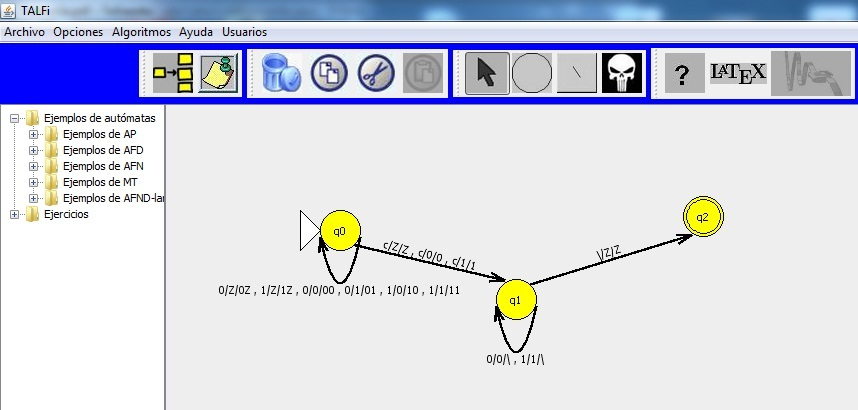
\includegraphics[width=\textwidth]{apd.jpg}
\end{center}


\subsection{Gram\'atica independiente de contexto}
Una gram\'atica independiente de contexto es una notaci\'on formal que sirve para expresar las definiciones recursivas de los lenguajes. Una gram\'atica consta de una o m\'as variables que representan las clases de cadenas, es decir, los lenguajes. Existen reglas que establecen c\'omo se construyen las cadenas de cada clase. La construcci\'on puede emplear s\'imbolos del alfabeto, cadenas que se sabe que pertenecen a una de las clases, o ambos elementos.

\begin{itemize}
\item Defini\'on formal:\\
Existen cuatro componentes importantes en una descripci\'on gramatical de un lenguaje:
\begin{enumerate}
\item Un conjunto finito de s\'imbolos que forma las cadenas del lenguaje que se est\'a definiendo. Denominamos a este conjunto alfabeto terminal o alfabeto de s\'imbolos terminales.\\
\item Un conjunto finito de variables, denominado tambi\'en en ocasiones s\'imbolos no terminales o categor\'ias sint\'acticas. Cada variable representa un lenguaje; es decir, un conjunto de cadenas.\\
\item Una de las variables representa el lenguaje que se est\'a definiendo; se denomina s\'imbolo inicial. Otras variables representan las clases auxiliares de cadenas que se emplean para definir el lenguaje del s\'imbolo inicial.
\item Un conjunto finito de producciones o reglas que representan la definici\'on recursiva de un lenguaje. Cada producci\'on consta de:\\
\begin{itemize}
\item Una variable a la que define (parcialmente) la producci\'on. Esta variable a menudo se denomina cabeza de producci\'on.\\
\item El s\'imbolo de producci\'on $\rightarrow$ . \\
\item Una cadena formada por cero o m\'as s\'imbolos terminales y variables. Esta cadena, denominada cuerpo de la producci\'on, representa una manera de formar cadenas pertenecientes al lenguaje de la variable de la cabeza. De este modo, dejamos los s\'imbolos terminales invariables y sustituimos cada una de las variables del cuerpo por una cadena que sabemos que pertenece al lenguaje de dicha variable.\\
\end{itemize}
\end{enumerate}

Los cuatro componentes que acabamos de describir definen una gram\'atica independiente de contexto (GIC), o simplemente una gram\'atica. Representamos una gram\'atica independiente de contexto G mediante sus cuatro componentes, es decir, G=(V,T,P,S), donde V es el conjunto de variables, T son los s\'imbolos terminales, P es el conjunto de producciones y S es el s\'imbolo inicial.

\item Ejemplos:
\begin{enumerate}
\item Una simple gram\'atica independiente de contexto es
\begin{center}
    S $\rightarrow$ aSb $\mid$ $\epsilon$\\
\end{center}
donde $\mid$ es un ``o'' l\'ogico y es usado para separar m\'ultiples opciones para el mismo s\'imbolo no terminal, $\epsilon$ indica una cadena vac\'ia.\\Esta gram\'atica genera el lenguaje no regular \{$a^{n} b^{n}$: n $\ge$ 0 \} .\\
\item Aqu\'i hay una gram\'atica independiente de contexto para expresiones enteras algebraicas sint\'acticamente correctas sobre las variables algebraicas, que son s\'imbolos terminales en la gram\'atica, x, y, z:
\begin{center}
    S $\rightarrow$ x $\mid$ y $\mid$ z $\mid$ S + S $\mid$ S - S $\mid$ S *S $\mid$ S/S $\mid$ (S)
\end{center}
Generar\'ia, por ejemplo, la cadena (x + y) *x - z *y / (x + x)\\
\item Una gram\'atica independiente de contexto para un lenguaje consistente en todas las cadenas que se pueden formar con las letras a y b, habiendo un n\'umero diferente de una que de otra, ser\'ia:\\

    S $\rightarrow$ U $\mid$ V\\
    U $\rightarrow$ TaU $\mid$ TaT\\
    V $\rightarrow$ TbV $\mid$ TbT\\
    T $\rightarrow$ aTbT $\mid$ bTaT $\mid$ $\epsilon$\\

T genera todas las cadenas con la misma cantidad de letras a que b, U genera todas las cadenas con m\'as letras a, y V todas las cadenas con m\'as letras b.\\
\item Otro ejemplo para un lenguaje es \{$a^{n} b^{m} c^{m+n}$: n $\ge$ 0, m $\ge$ 0 \} . No es un lenguaje regular, pero puede ser generado por la siguiente gram\'atica independiente de contexto.\\

    S  $\rightarrow$ aSc $\mid$ B\\
    B $\rightarrow$ bBc $\mid$ E\\
\end{enumerate}
\item Formas normales:
\begin{itemize}
\item Forma normal de Greibach:\\
\newline
Una gram\'atica independiente de contexto (GIC) est\'a en forma normal de Greibach (FNG) si todas y cada una de sus reglas de producci\'on tienen un consecuente que empieza por un car\'acter del alfabeto, tambi\'en llamado s\'imbolo terminal. Formalmente, cualquiera de las reglas tendr\'a la estructura:\\
\begin{center}
A $\rightarrow$ aw
\end{center}
Donde ``A'' es el antecedente de la regla, que en el caso de las GIC debe ser necesariamente un solo s\'imbolo auxiliar. Por su parte, ``a'' es el mencionado comienzo del consecuente y, por tanto, un s\'imbolo terminal. Finalmente, ``w'' representa una concatenaci\'on gen\'erica de elementos gramaticales, esto es, una sucesi\'on exclusivamente de auxiliares, inclusive, pudiera ser la palabra vac\'ia; en este caso particular, se tendr\'ia una regla llamada "terminal":\\
\begin{center}
A $\rightarrow$ a
\end{center}
Existe un teorema que prueba que cualquier GIC, cuyo lenguaje no contiene a la palabra vac\'ia, si no lo est\'a ya, se puede transformar en otra equivalente que s\'i est\'e en FNG. Para su demostraci\'on, normalmente, se procede por construcci\'on, es decir, se plantea directamente un algoritmo capaz de obtener la FNG a partir de una GIC dada.\\
\item Forma normal de Chomsky:\\
\newline
Una gram\'atica formal est\'a en forma normal de Chomsky si todas sus reglas de producci\'on son de alguna de las siguientes formas:
\begin{center}
A $\rightarrow$ BC \'o\\ 
A $\rightarrow$ a\\
\end{center}
donde A, B y C son s\'imbolos no terminales (o variables) y a es un s\'imbolo terminal.
Todo lenguaje independiente de contexto que no posee a la cadena vac\'ia, es expresable por medio de una gram\'atica en forma normal de Chomsky (FNC) y rec\'iprocamente. Adem\'as, dada una gram\'atica independiente de contexto, es posible algor\'itmicamente producir una FNC equivalente, es decir, que genera el mismo lenguaje.
\end{itemize}
\end{itemize}
\subsection{Lenguaje independiente de contexto}
Un lenguaje independiente de contexto es aquel generado por una gram\'atica \htmladdnormallink{independiente de contexto.}{http://es.wikipedia.org/wiki/Gramatica_independiente_de_contexto} Estos conceptos pertenecen a un \'area de la Ciencia de la
Computaci\'on llamada Computaci\'on Te\'orica.\\
Los lenguajes de programaci\'on son lenguajes independientes del contexto. Existe una forma mec\'anica de convertir la descripci\'on de un lenguaje como GIC en un analizador sint\'actico: el componente del compilador descubre la estructura del programa fuente y representa dicha estructura mediante un arbol de derivaci\'on.\\
Otro ejemplo es el lenguaje HTML, o tambi\'en el lenguaje XML, cuya parte fundamental es la DTD (Document Type Definition, definici\'on de tipo de documento), que principalmente es una gram\'atica independiente de contexto que describe las etiquetas permitidas y las formas en que dichas etiquetas pueden anidarse.

\subsection{M\'aquina de Turing}
\begin{itemize}
\item Descripci\'on:\\
\newline
La m\'aquina de Turing es un modelo computacional introducido por Alan Turing en el trabajo ``On computable numbers, with an application to the Entscheidungsproblem'', publicado por la Sociedad Matem\'atica de Londres en 1936, en el cual se estudiaba la cuesti\'on planteada por David Hilbert sobre si las matem\'aticas son decidibles, es decir, si hay un m\'etodo definido que pueda aplicarse a cualquier sentencia matem\'atica y que nos diga si esa sentencia es cierta o no. Turing ide\'o un modelo formal de computador, la m\'aquina de Turing, y demostr\'o que exist\'ian problemas que una m\'aquina no pod\'ia resolver. La m\'aquina de Turing es un modelo matem\'atico abstracto que formaliza el concepto de \htmladdnormallink{algoritmo.}{http://es.wikipedia.org/wiki/Algoritmo}\\

La m\'aquina de Turing consta de un cabezal lector/escritor y una cinta infinita en la que el cabezal lee el contenido, borra el contenido anterior y escribe un nuevo valor. Las operaciones que se pueden realizar en esta m\'aquina se limitan a:
\begin{center}
\begin{enumerate}
\item avanzar el cabezal lector/escritor hacia la derecha.
\item avanzar el cabezal lector/escritor hacia la izquierda.
\end{enumerate}
\end{center}
El c\'omputo es determinado a partir de una tabla de estados de la forma:
\begin{center}
(estado, valor) $\rightarrow$ (nuevo estado, nuevo valor, direcci\'on)\\
\end{center}
Esta tabla toma como par\'ametros el estado actual de la m\'aquina y el car\'acter le\'ido de la cinta, dando la direcci\'on para mover el cabezal, el nuevo estado de la m\'aquina y el valor a ser escrito en la cinta.

Con este aparato extremadamente sencillo es posible realizar cualquier c\'omputo que un computador digital sea capaz de realizar.

Mediante este modelo te\'orico y el an\'alisis de \htmladdnormallink{complejidad}{http://es.wikipedia.org/wiki/Complejidad_computacional} de algoritmos, fue posible la categorizaci\'on de problemas computacionales de acuerdo a su comportamiento, apareciendo as\'i, el conjunto de problemas denominados \htmladdnormallink{P}{http://es.wikipedia.org/wiki/Tiempo_polinomico} y \htmladdnormallink{NP}{http://es.wikipedia.org/wiki/NP_(Complejidad_computacional)}, cuyas soluciones en tiempo polin\'omico son encontradas seg\'un el determinismo y no determinismo respectivamente de la m\'aquina de Turing.

De hecho, se puede probar matem\'aticamente que para cualquier programa de computadora es posible crear una m\'aquina de Turing equivalente. Esta prueba resulta de la tesis de Church-Turing, formulada por Alan Turing y Alonzo Church, de forma independiente a mediados del siglo XX.

La idea subyacente es el concepto de que una m\'aquina de Turing es una persona ejecutando un procedimiento efectivo definido formalmente, donde el espacio de memoria de trabajo es ilimitado, pero en un momento determinado s\'olo una parte finita es accesible. La memoria se divide en espacios de trabajo denominados celdas, donde se pueden escribir y leer s\'imbolos. \newline Inicialmente todas las celdas contienen un s\'imbolo especial denominado ``blanco''. Las instrucciones que determinan el funcionamiento de la m\'aquina tienen la forma, ``si estamos en el estado x leyendo la posici\'on y, donde hay escrito el s\'imbolo z, entonces este s\'imbolo debe ser reemplazado por este otro s\'imbolo, y pasar a leer la celda siguiente, bien a la izquierda o bien a la derecha''.
\newline La m\'aquina de Turing puede considerarse como un aut\'omata capaz de reconocer lenguajes formales. En ese sentido es capaz de reconocer los lenguajes recursivamente enumerables, de acuerdo a la jerarqu\'ia de Chomsky. Su potencia es, por tanto, superior a otros tipos de aut\'omatas, como el aut\'omata finito, o el aut\'omata con pila, o igual a otros modelos con la misma potencia computacional.
\item Nociones preliminares: \\
\newline
Podemos imaginarnos una m\'aquina de Turing de la manera siguiente: la m\'aquina
consta de una unidad de control, que puede estar en cualquier estado tomado de un
conjunto finito. Hay una cinta dividida en casillas, que puede contener un s\'imbolo,
tomado de otro conjunto finito.
\begin{center}
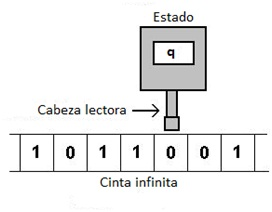
\includegraphics{turi1.jpg}
\end{center}
Inicialmente, se sit\'ua en la cinta de entrada, que es una cadena de s\'imbolos de
longitud finita, elegidos del alfabeto de entrada. El resto de las casillas de la cinta,
que se extiende infinitamente hacia la derecha y la izquierda, contiene, inicialmente,
un s\'imbolo denominado espacio en blanco.\\ El espacio en blanco es un s\'imbolo de
cinta, pero no un s\'imbolo de entrada, y puede haber tambi\'en otros s\'imbolos de
cinta adem\'as de los s\'imbolos de entrada y del espacio en blanco.\\
Existe una cabeza de cinta que siempre est\'a situada sobre una de las casillas de
la cinta. Se dice que la m\'aquina de Turing est\'a se\~nalando dicha casilla. Al
principio, la cabeza de la cinta se encuentra en la casilla de entrada que se encuentra
m\'as a la izquierda y no es un blanco.\\
Un movimiento de la m\'aquina de Turing es una funci\'on del estado de la unidad de
control, del s\'imbolo de la cinta y de la direcci\'on. En un movimiento, la m\'aquina de
Turing:
\begin{enumerate}
\item Cambiar\'a de estado. Opcionalmente, el siguiente estado puede ser el mismo
que el actual.
\item Escribir\'a un s\'imbolo de cinta en la casilla se\~nalada por la cabeza. Este
s\'imbolo de cinta sustituye al s\'imbolo que estuviera anteriormente en la casilla.
Opcionalmente, el s\'imbolo escrito puede ser el mismo que hab\'ia en dicha casilla.
\item Mover\'a la cabeza de la cinta hacia la izquierda o hacia la derecha. En nuestro
formalismo, no se exige que haya un movimiento, y se permite que la cabeza
permanezca en el mismo lugar.
\end{enumerate}
\newpage
\item Definici\'on formal de una m\'aquina de Turing:\\
\newline
La notaci\'on formal que utilizaremos para una m\'aquina de Turing es similar a la
utilizada para los aut\'omatas finitos o para los aut\'omatas de pila.\\
M = ($\mathcal{Q}$,$\Sigma$,$\Gamma$,$\delta$,$q_{0}$,\#,F)
cuyas componentes tienen el siguiente significado:
\begin{itemize}
\item $\mathcal{Q}$: El conjunto finito de estados de la unidad de control.
\item $\Sigma$: El conjunto finito de s\'imbolos de entrada.
\item $\Gamma$: El conjunto completo de s\'imbolos de cinta; $\Sigma$ siempre es un
subconjunto de $\Gamma$.
\item $\delta$: La funci\'on de transici\'on. Los argumentos de $\delta$(q,X) son un
estado q y un s\'imbolo de cinta X. El valor de $\delta$(q,X), si est\'a definido, es una
tupla (p,Y,S), donde:
\begin{enumerate}
\item p es el estado siguiente de $\mathcal{Q}$.
\item Y es el s\'imbolo de $\Gamma$, que se escribe en la casilla se\~nalada por la
cabeza de la cinta y que sustituye al s\'imbolo que se encontraba en dicha casilla.
\item S es un sentido, I, D o N (``izquierda'', ``derecha'' o ``ninguno'' respectivamente),
que nos indica el sentido en el que se mueve la cabeza.
\end{enumerate}
\item $q_{0}$: El estado inicial (uno de los elementos de $\mathcal{Q}$) en el cual se encuentra
inicialmente la unidad de control.
\item \#: El s\'imbolo de espacio en blanco. Este s\'imbolo forma parte de $\Gamma$
pero no de $\Sigma$; es decir, no es un s\'imbolo de entrada. El espacio en blanco
aparece inicialmente en todas las casillas de la cinta, excepto en aqu\'ellas que
contienen los s\'imbolos de la entrada.
\item F: El conjunto de estados finales o de aceptaci\'on, que constituye un
subconjunto de $\mathcal{Q}$.
\end{itemize}





\item Ejemplo:\\
\newline
Definimos una m\'aquina de Turing sobre el alfabeto \{0,1\}, donde 0 representa el s\'imbolo blanco. La m\'aquina comenzar\'a su proceso situada sobre un s\'imbolo ``1'' de una serie. La m\'aquina de Turing copiar\'a el n\'umero de s\'imbolos ``1'' que encuentre hasta el primer blanco detr\'as de dicho s\'imbolo blanco. Es decir, situada sobre el 1 situado en el extremo izquierdo, doblar\'a el n\'umero de s\'imbolos 1, con un 0 en medio. As\'i, si tenemos la entrada ``111'' devolver\'a ``1110111'', con ``1111'' devolver\'a ``111101111'', y sucesivamente.\\
El conjunto de estados es \{$q_1$, $q_2$, $q_3$, $q_4$, $q_5$\} y el estado inicial es $q_1$.\\
\newline
La tabla que describe la funci\'on de transici\'on es la siguiente:\\
\begin{center}
\begin{tabular}{||c|c|c|c|c||}
\hline
Estado & S\'imbolo le\'ido & S\'imbolo escrito & Mov. & Estado sig. \\
\hline
$q_{1}$ & 1 & 0 & D & $q_{2}$ \\
\hline
$q_{1}$ & 1 & 0 & D & $q_{2}$ \\
\hline
$q_{2}$ & 1 & 1 & D & $q_{2}$ \\
\hline
$q_{2}$ & 0 & 0 & D & $q_{3}$ \\
\hline
$q_{3}$ & 0 & 1 & I & $q_{4}$ \\
\hline
$q_{3}$ & 1 & 1 & D & $q_{3}$ \\
\hline
$q_{4}$ & 1 & 1 & I & $q_{4}$ \\
\hline
$q_{4}$ & 0 & 0 & I & $q_{5}$ \\
\hline
$q_{5}$ & 1 & 1 & I & $q_{5}$ \\
\hline
$q_{5}$ & 0 & 1 & D & $q_{1}$ \\
\hline
\end{tabular}
\end{center}

El funcionamiento de una computaci\'on de esta m\'aquina se puede mostrar con el siguiente ejemplo (en negrita se resalta la posici\'on de la cabeza lectora/escritora):\\
\begin{center}
\begin{tabular}{||c|c|c||}
\hline
Paso & Estado & Cinta\\
\hline
1 & $q_{1}$ & $\bf{1}$1\\
\hline
2 & $q_{2}$ & 0$\bf{1}$\\
\hline
3 & $q_{2}$ & 01$\bf{0}$\\
\hline
4 & $q_{3}$ & 010$\bf{0}$\\
\hline
5 & $q_{4}$ & 01$\bf{0}$1\\
\hline
6 & $q_{5}$ & 0$\bf{1}$01\\
\hline
7 & $q_{5}$ & $\bf{0}$101\\
\hline
8 & $q_{1}$ & 1$\bf{1}$01\\
\hline
9 & $q_{2}$ & 10$\bf{0}$1\\
\hline
10 & $q_{3}$ & 100$\bf{1}$\\
\hline
11 & $q_{3}$ & 1001$\bf{0}$\\
\hline
12 & $q_{4}$ & 100$\bf{1}$1\\
\hline
13 & $q_{4}$ & 10$\bf{0}$11\\
\hline
14 & $q_{5}$ & 1$\bf{0}$011\\
\hline
15 & $q_{1}$ & 11$\bf{0}$11\\
\hline
Parada & &\\
\hline
\end{tabular}
\end{center}

La m\'aquina realiza su proceso por medio de un bucle, en el estado inicial q1, reemplaza el primer 1 con un 0, y pasa al estado q2, con el que avanza hacia la derecha, saltando los s\'imbolos 1 hasta un 0 (que debe existir), cuando lo encuentra pasa al estado q3, con este estado avanza saltando los 1 hasta encontrar otro 0 (la primera vez no habr\'ia ning\'un 1). Una vez en el extremo derecho, a\~nade un 1. Despu\'es comienza el proceso de retorno; con q4 vuelve a la izquierda saltando los 1, cuando encuentra un 0 (en el medio de la secuencia), pasa a q5 que contin\'ua a la izquierda saltando los 1 hasta el 0 que se escribi\'o al principio. Se reemplaza de nuevo este 0 por 1, y pasa al s\'imbolo siguiente, si es un 1, se pasa a otra iteraci\'on del bucle, pasando al estado q1 de nuevo. Si es un s\'imbolo 0, ser\'a el s\'imbolo central, con lo que la m\'aquina se detiene al haber finalizado su c\'omputo.
\end{itemize}
\subsection{Algoritmo CYK\\}
El algoritmo de Cocke-Younger-Kasami (CYK) determina si una cadena puede ser generada por una gram\'atica independiente de contexto y, si es posible, c\'omo puede ser generada. Este proceso es conocido como an\'alisis sint\'actico de la cadena. 

La versi\'on est\'andar CYK reconoce lenguajes definidos por una gram\'atica independiente de contexto escrita en la forma normal de Chomsky. Cualquier gram\'atica independiente de contexto puede ser convertida a FNC sin mucha dificultad, CYK puede usarse para reconocer cualquier palabra de lenguaje independiente de contexto.\\

Consiste en crear una tabla, de tama\~{n}o como la cadena a reconocer, siempre que la cadena sea distinta de $\epsilon$, pues en ese caso solo basta comprobar si es una producci\'on de la variable inicial. Cada celda la rellenamos con la lista de variables que nos pueden permitir crear las subcadenas basadas en la cadena dada, hasta que llegamos a la celda de la primera columna y la fila de la longitud de la cadena. Si \'esta contiene a la variable inicial, es que a partir de ella podr\'iamos derivar la cadena original, y por tanto ser\'ia reconocida por la gram\'atica, y en consecuencia por el aut\'omata de pila.\\

En el peor caso asint\'otico la complejidad temporal de CYK es c\'ubica sobre la longitud de la cadena analizada. Esto hace a \'este algoritmo uno de los m\'as eficientes en el reconocimiento de cadenas de los lenguajes independientes de contexto.\\ \newline \newline

Podemos ver una codificaci\'on simplificada en pseudoc\'odigo del algoritmo:\\
\begin{itemize}
\item \noindent Entrada : G=(V, T, P, S) en FNC y w = $w_{1}$ $w_{2}$ \ldots $w_{n}$ (w$\neq$ $\epsilon$)

\item \noindent Salida : Cierto (si w $\in$ L(G)) o Falso (si w $\notin$ L(G))

 \item \noindent M\'etodo :
\end{itemize}
{\ttfamily

\noindent Para i=1 hasta n\\

\indent $V_{i1}$ = \{ A : A $\rightarrow$ $w_{i}$ $\in$ P \}\\

finPara\\

Para j=2 hasta n\\

\indent Para i=1 hasta n-j+1\\

\indent \indent $V_{ij}$ = $\emptyset$\\

\indent \indent Para k=1 hasta j-1\\

\indent \indent \indent $V_{ij}$ = $V_{ij}$ $\cup$ \{ A : A $\rightarrow$ BC $\in$ P, B $\in$ $V_{ik}$, C $\in$ $V_{i+k}$, j-k \}\\

\indent \indent finPara\\

\indent finPara\\

finPara\\

Si S $\in$ $V_{1n}$ devolver Cierto\\

sino devolver Falso\\

}

\newpage

\section{Lenguaje generado por un aut\'omata de pila}
Esta parte fue la que nos llev\'o m\'as tiempo, pues como hemos explicado antes, seguimos una l\'inea de trabajo que desafortunadamente nos llevo a un callej\'on sin salida. Nos centramos en palabras que pertenec\'ian al lenguaje, punto importante pero no el vital para el que sirven los aut\'omatas: definir un lenguaje.

\subsection{Pasos de simplificaci\'on antes y despu\'es de realizar transformaciones FNC o FNG}

Estamos acostumbrados en los ejemplos a ver gram\'aticas con pocos s\'imbolos de variable, y en general bastante simplificadas. Al aplicar el algoritmo que nos da la gram\'atica independiente de contexto asociada, vimos que a\'un teniendo pocos estados, en el momento que el n\'umero de aristas comienza a crecer, obtenemos unas gram\'aticas bastante grandes, y nos vimos en la obligaci\'on de reducirlas adaptando las reglas de simplificaci\'on de una gram\'atica:\\
\begin{itemize}

\item Eliminaci\'on de variables sin producciones.

\item Sustituci\'on de una variable por su producci\'on si s\'olo tiene asociada a ella una \'unica producci\'on y es $\epsilon$.

\item Sustituci\'on de una variable por su producci\'on si s\'olo tiene asociada a ella una \'unica producci\'on.

\item Eliminaci\'on de producciones para variables inalcanzables.

\item Eliminaci\'on de producciones $\epsilon$ que cuya cabeza no sea la variable inicial.

\item Renombramiento de variables.
\end{itemize}

Las tres primeras normas se aplican antes de comentar la transformaci\'on en forma normal de una gram\'atica. Nos permiten reducir y dejar mucho m\'as claro el lenguaje que definen. Las dos siguientes las aplicamos para simplificar el resultado final, pues las formas normales tienen unas caracter\'isticas estrictas, por tanto en algunos casos no har\'a ni falta aplicarlas, y en otros es necesario porque no se aplicaron al principio.

A continuaci\'on mostramos algunos de estos resutados que aparecen en el archivo HTML que se genera con la simplificaci\'on de gram\'aticas independientes de contexto.\\
\begin{center}
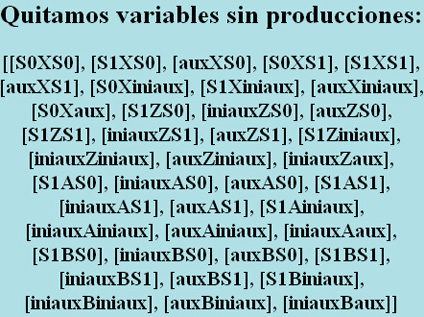
\includegraphics[scale=0.5]{varsinprod.jpg} \newline
\end{center}
\begin{center}
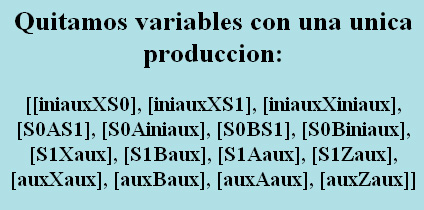
\includegraphics[scale=0.5]{varunaprod.jpg} \newline
\end{center}
\begin{center}
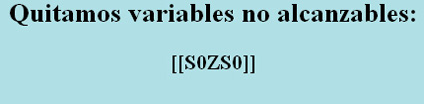
\includegraphics[scale=0.5]{varnoalc.jpg} \newline
\end{center}


Puede verse una breve descripci\'on del paso de simplificaci\'on a realizar, y sobre que variables se hace, y a continuaci\'on mostramos la gram\'atica resultante. As\'i hasta renombrar las variables para que la gram\'atica quede a la forma en la que estamos habituados a tratar.

\begin{center}
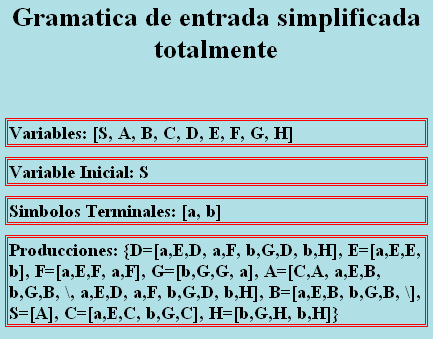
\includegraphics[scale=0.5]{entradafinsimp.jpg}\\
\end{center}

\subsection{Algoritmo de paso de AP $\rightarrow$ gram\'atica\\}
Encontramos muchas dificultades, pues este algoritmo viene detallado muy formalmente y los ejemplos que pudimos encontrar no eran demasiado aclaratorios.
Para realizar esta nueva funci\'on, hemos incluido en el men\'u de algoritmos el bot\'on ``Simplificaci\'on GIC'':\\
\begin{center}
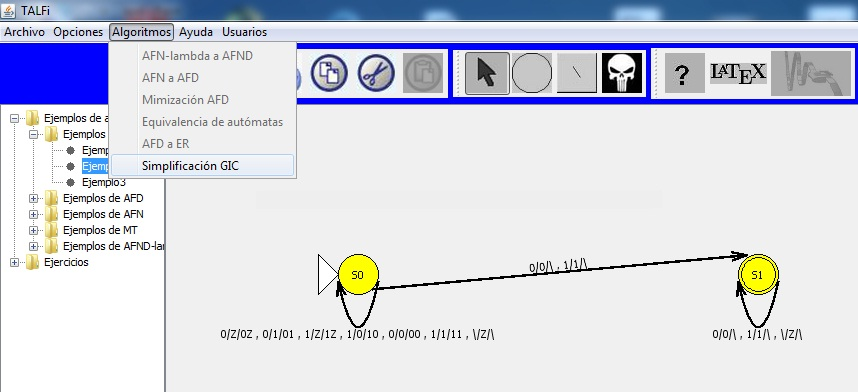
\includegraphics[width=\textwidth]{auto4.jpg}\newline
\end{center}
En primer lugar, tenemos que distinguir si el aut\'omata de pila tiene estados finales o no. Si se da el primer caso, tenemos que convertir el aut\'omata dado en otro equivalente que reconozca el mismo lenguaje por pila vac\'ia que por estado final. Para ello, seguimos el algoritmo que nos dice c\'omo hacerlo:
\begin{itemize}
\item Se debe incluir un nuevo estado inicial y un nuevo fondo de pila. Se a\~nade una transici\'on vac\'ia que vaya al estado inicial antiguo, que apile el antiguo fondo de pila sobre el nuevo.

\item Se incluye un nuevo estado, que ser\'a donde se proceda a desapilar todos los s\'imbolos que pudiera haber apilados en el momento de aceptaci\'on de la cadena cuando era aceptada por estado final. Se a\~nade una transici\'on vac\'ia desde cada estado final que desapile para cada s\'imbolo del alfabeto de pila y que vaya al nuevo estado. Por \'ultimo, en este nuevo estado existir\'an aristas con las mismas caracter\'isticas que las anteriores. As\'i, nos aseguramos que, sea posible la transici\'on o no, se desapilar\'ia siempre la pila.
\end{itemize}

\begin{center}
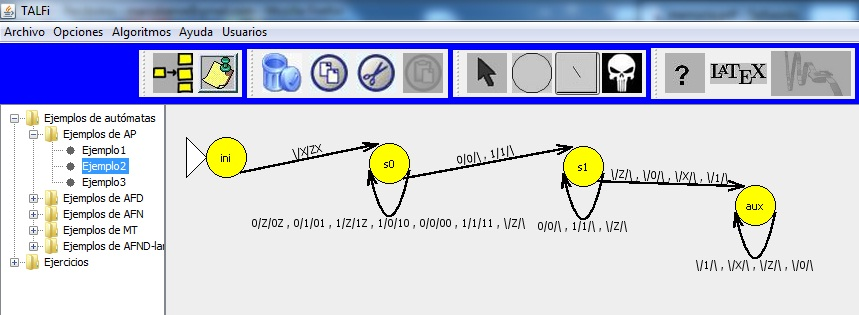
\includegraphics[width=\textwidth]{roci1.jpg}
\end{center}

En ning\'un caso modificamos el aut\'omata que dibuje el usuario, haremos una copia de \'el. Creemos que no es necesario porque es una conversi\'on necesaria para ejecutar el algoritmo, y es bastante intuitivo el cambio, pero si en un futuro se desea se podr\'ia sustituir el original por el nuevo calculado a partir de \'el.\\

Una vez que tenemos el aut\'omata libre de estados finales, aplicamos el algoritmo que nos convierte un aut\'omata de pila en una gram\'atica independiente del contexto. Consiste en lo siguiente:
\begin{itemize}
\item El s\'imbolo inicial de la gram\'atica ser\'a S. Para cada estado p del aut\'omata, siendo $q_{0}$ el estado inicial tendremos la producci\'on\\ S $\rightarrow$ [$q_{0}$Zp]
\item Si existe una transici\'on tal que desapile la cima de la pila,\\ $\delta$(p,Z,a) = (q, $\epsilon$),
a\~nadimos la producci\'on [pZq] $\rightarrow$ a. Esta a puede ser tambi\'en $\epsilon$.
\item Por \'ultimo, para transiciones $\delta$(p,Z,a) = (q,$A_{1}A_{2}$ \ldots $A_{n}$), debemos construir todas las listas de estados de longitud n, y crear para cada lista la producci\'on:
[pZ$r_{k}$]= a[q$A_{1}r_{1}$][$r_{2}A_{2}r_{3}$] \ldots [$r_{k-1}A_{n}r_{k}$]. Aqu\'i a tambi\'en puede ser $\epsilon$.
\end{itemize}
Una vez que tenemos la gram\'atica, la simplificamos, pues en muchos casos ayuda a reducir los s\'imbolos de variable. Sustituimos todas las variables con producciones unitarias excepto con la variable inicial, y eliminamos las producciones que sean vac\'ias siempre y cuando no aparezcan en S. Para hacer m\'as f\'acil al usuario el entender la gram\'atica, cambiamos los s\'imbolos de producci\'on, que hasta el momento eran del tipo [qZp], por letras may\'usculas del abecedario. Creemos que es bastante grande y que no es probable que ninguna gram\'atica rebase ese n\'umero de variables.

\subsection{Algoritmo de simplificaci\'on gram\'atica independiente de contexto a FNG}
Cuando ya tenemos la gram\'atica simplificada podemos dedicarnos a convertirla en una gram\'atica de Greibach. Se caracteriza porque las producciones empiezan por un s\'imbolo terminal, como ya sabemos.\\ 
Para poder localizar que variables tienen producciones que comiencen por otra variable, construimos una tabla cuyas filas y columnas son las variables de la gram\'atica. Si alguna producci\'on de las variables de las filas comienza con alguna de las variables de las columnas, marcamos la casilla correspondiente.\\ 
Ve\'amoslo paso por paso, para el ejemplo de la \'ultima imagen:\\

La gram\'atica que nos genera este aut\'omata, es la siguiente:\\
\newline
\begin{center}
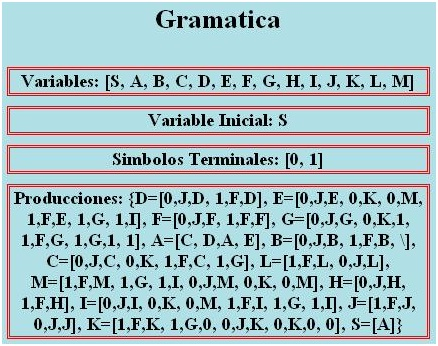
\includegraphics[scale=0.7]{gram1.jpg}
\end{center}

Y la tabla que se genera tal y como hemos dicho antes es:
\newline
\begin{center}
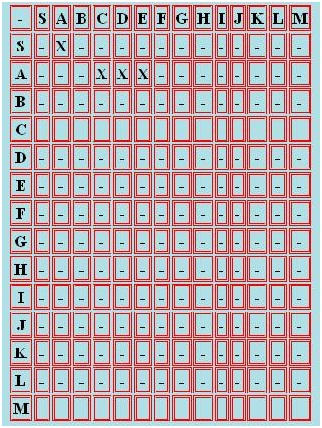
\includegraphics[scale=0.5]{gram2.jpg}
\end{center}


Y mientras que no marquemos una casilla diagonal, es sencillo. Selecciona-\\mos las casillas de la columna m\'as a la izquierda, y sustituimos creando producciones nuevas de la variable marcada en la columna, incluy\'endolas en la variable de la fila. Este proceso es autom\'atico y no se muestra al usuario por pasos, se le vuelve a mostrar la gram\'atica resultante de las sustituciones:\\
\newline 
\begin{center}
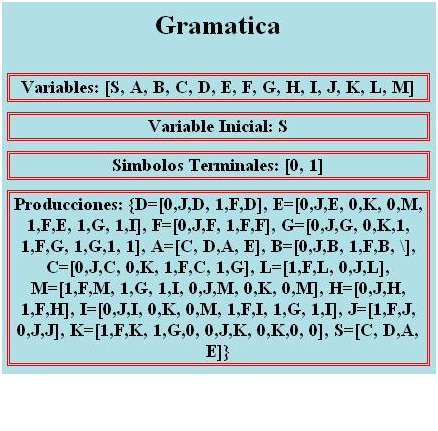
\includegraphics[scale=0.6]{gram3.jpg}\\
\end{center}


Y volvemos a generar la tabla, hasta que llegamos a un punto que la tabla no est\'a marcada, y eso quiere decir que ya est\'a en forma normal de Greibach.\\
\newline

\begin{center}
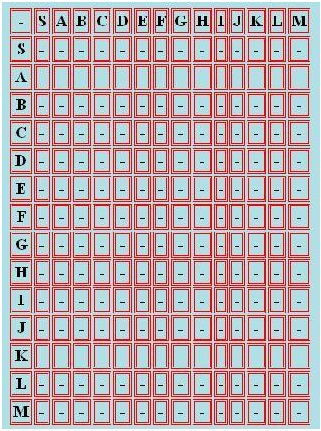
\includegraphics[scale=0.6]{gram4.jpg}\\
\end{center}


Momento en el que ya hemos terminado y devolvemos la gram\'atica final:\\
\newline
\begin{center}
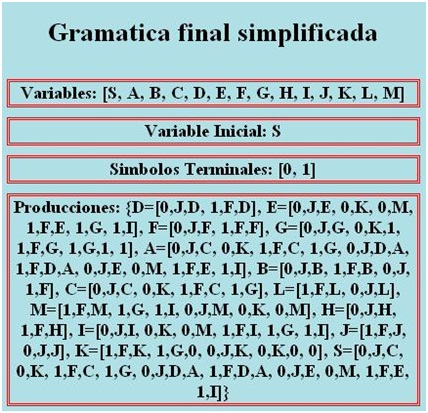
\includegraphics[scale=0.6]{gram5.jpg}\\
\end{center}

A esta gram\'atica que devolvemos como final, le aplicamos otro algoritmo de simplificaci\'on, el de eliminar las producciones vac\'ias siempre que no sean producciones de la variable inicial. 
Este algoritmo consiste en lo siguiente:
\begin{enumerate}
\item Localizamos que variables, siempre que no sea la inicial, tiene una producci\'on vac\'ia. Eliminamos la producci\'on vac\'ia de sus producciones para cada una de las variables que cumplan esta caracter\'istica.
\item Buscamos en el resto de las producciones de las variables si existe alguna que contenga la variable con la producci\'on vac\'ia. La sustituimos, y la a\~nadimos a la lista de producciones.
\item Nos deshacemos de variables que no fueran alcanzables desde el s\'imbolo inicial, repitiendo el proceso para comprobar si su eliminaci\'on ha provocado alg\'un cambio en la gram\'atica.
\end{enumerate}
Consideramos que cuando la tabla no contiene marcas es el momento ideal de proceder a eliminarlas, porque si lo hacemos antes de que est\'e en forma normal de Greibach, no podemos asegurar que entremos en un bucle infinito y no podamos salir de \'el. Por ejemplo:\\
Tenemos dos producciones del tipo:\\
\begin{center}
A $\rightarrow$ \ldots $\mid$ E $\mid$ $\epsilon$ $\mid$ \ldots\\
E $\rightarrow$ \ldots $\mid$ A $\mid$ \ldots\\
\end{center}
Siendo A, E variables de la gram\'atica. Si eliminamos las producciones vac\'ias, ocurrir\'ia lo siguiente:\\
\begin{enumerate}	
\item Sustituimos  las apariciones de A por $\epsilon$. Obtendr\'iamos lo siguiente:\\
\begin{center}
	A $\rightarrow$ \ldots $\mid$ E $\mid$ \ldots\\
	E $\rightarrow$ \ldots $\mid$ $\epsilon$ $\mid$ \ldots\\
\end{center}
\item Volver\'iamos a estar en la misma situaci\'on, pues seguimos teniendo una variable con una producci\'on vac\'ia.
\end{enumerate}
Este problema no lo tenemos si la gram\'atica tiene la forma normal de Greibach, pues nos aseguramos que el primer s\'imbolo de la producci\'on es un terminal, y nunca ocurrir\'a el caso anterior. 

Por otro lado, puede ocurrir que se marque una casilla que est\'e en la diagonal de la tabla. En ese caso el proceso es algo m\'as delicado, pues hemos de incluir una nueva variable, ya que existe recursividad y por mucho que se sustituya una y otra vez no podr\'iamos eliminarla.


\subsection{Algoritmo de simplificaci\'on gram\'atica independiente de contexto a FNC\\}
Ya que hemos incluido simplificaciones de gram\'atica, no podemos no incluir otras de las simplificaciones, quiz\'a m\'as importante incluso que la forma normal de Greibach: La forma normal de Chomsky.\\
\newline
Convertir una gram\'atica en forma normal de Chomsky, consiste en dos pasos muy sencillos. En primer lugar, una gram\'atica est\'a en forma normal de Chomsky si las producciones son del tipo:
\begin{center}
A $\rightarrow$ BC 	Siendo A, B, C $\in$ V\\
A $\rightarrow$ a        Siendo a $\in$  T
\end{center}
Y s\'olo se puede incluir la producci\'on S $\rightarrow$ $\epsilon$ si S no aparece en ninguna de las producciones del resto de variables y, por supuesto,  aparece en los casos que \'unicamente $\epsilon$ es reconocida por la gram\'atica.\\
\newline
Con esta idea en la cabeza, es f\'acilmente entendible el algoritmo de transformaci\'on, que consta de dos fases:
\begin{itemize}
\item Fase 1: Para cada s\'imbolo terminal que pertenece a T, creamos producciones del tipo [Ca] $\rightarrow$ a
para todo a $\in$ T.
\begin{itemize}
\item Fase 1.1: Reemplazamos en todas las producciones las apariciones de s\'imbolos terminales  a por sus ``variables terminales'' [Ca] asociados que acabamos de crear.
\end{itemize}
\item Fase 2: Ahora tenemos que conseguir que las producciones est\'en formadas solamente por dos variables. Para ello procedemos de la siguiente manera:
\begin{itemize}
\item Fase 2.2: Recorremos todas las producciones. Si la longitud es mayor o igual a 3, esto es lo que hacemos:\\
Imaginemos que tenemos la siguiente producci\'on: A $\rightarrow$ $A_{1}A_{2}A_{3} \ldots A_{n}$. Creamos una nueva variable, [D0], que contendr\'a la producci\'on $A_{2}A_{3} \ldots A_{n}$, y modificamos la producci\'on que acabamos de encontrar suplant\'andola por A$\rightarrow$ $A_{1}$[D0].
\end{itemize}
	Esta fase 2 se repite hasta que todas las producciones tengan longitud menor que 3, o lo que es lo mismo, que ninguna cumpla la condici\'on para ser modificada.\\
\newline
En teor\'ia habr\'iamos acabado aqu\'i, pero puede ocurrir, que la gram\'atica original, tuviera producciones de s\'olo una variable, y entonces no estar\'ia la forma normal de Chomsky bien construida.\\ Este detalle en el algoritmo no se tiene en cuenta, pero es lo que nos ha ocurrido a lo largo de todo este a\~no trabajando en el proyecto:\\ las diferencias entre las aplicaciones te\'oricas, y lo que en la pr\'actica supone estudiar todos los casos, no \'unicamente el general, y buscar soluciones eficientes para devolver el resultado correcto. As\'i que, informalmente, a\~nadir\'iamos un tercer paso:
\item Fase 3: Si en alg\'un momento encontramos en las producciones alguna que consista en una variable, sustituimos esa variable por todas sus producciones, pues en principio tendr\'an la forma adecuada que requiere la forma normal de Chomsky. Y finalmente diremos que la gram\'atica est\'a simplificada en el momento que hayamos revisado todas las producciones y no hayamos hecho ninguna modificaci\'on.
\end{itemize}
A continuaci\'on, vamos a mostrar cu\'al es el resultado de obtener la forma normal de Chomsky en un aut\'omata sencillo:\\
\begin{center}
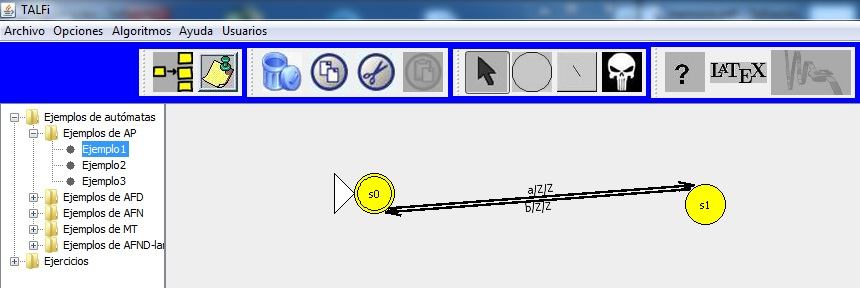
\includegraphics[width=\textwidth]{chom1.jpg}
\end{center}

Y la salida HTML mostrada con su forma normal de Chomsky, que tiene un formato id\'entico a la salida de la forma normal de Greibach excepto en los pasos que sigue para llegar al resultado final, es la siguiente:\\

\begin{enumerate}
\item Lo primero, saber cu\'al es la gram\'atica primigenia:\\
\begin{center}
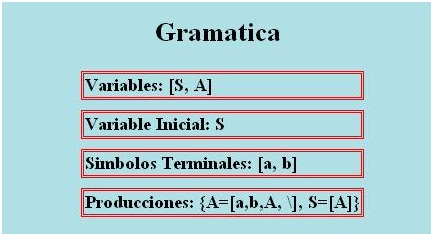
\includegraphics[scale=0.95]{chom2.jpg}
\end{center}
\item La salida obtenida de aplicar la primera fase, cuyo resultado es claramente intuitivo compar\'andolo con la gram\'atica original:\\
\begin{center}
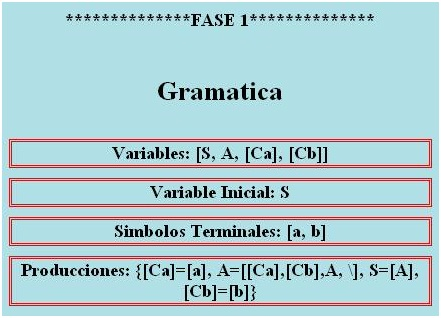
\includegraphics{chom3.jpg}
\end{center}

\item La salida obtenida de terminar con la segunda fase:\\
\begin{center}
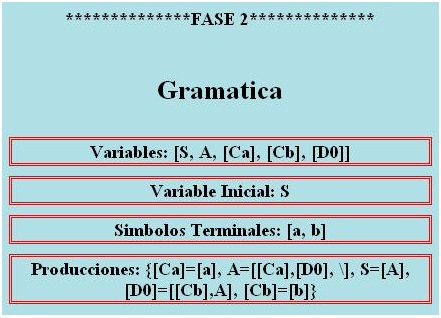
\includegraphics{chom4.jpg}
\end{center}
\item Observemos la producci\'on S $\rightarrow$ A y la producci\'on de [D0] c\'omo cambia al terminar con la simplificaci\'on y conseguir una gram\'atica en FNC:\\
\begin{center}
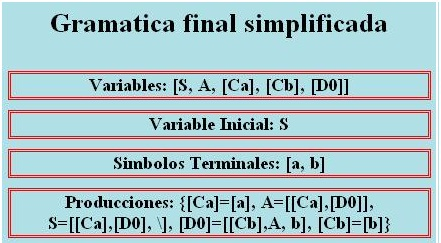
\includegraphics{chom5.jpg}
\end{center}
\end{enumerate}


\subsection{Generaci\'on aleatoria de palabras}
Como ya sabemos, los aut\'omatas de pila definen lenguajes. El uso de la pila dificulta en algunos casos saber c\'omo son las cadenas reconocidas, por tanto implementamos una manera de conseguir una lista que mostrase algunas de las palabras reconocidas.
Esta lista contiene como m\'aximo cinco palabras. En un primer momento pensamos en que tuviera diez, pero para gram\'aticas con muchas variables, es muy probable que tengan muchas producciones para cada una de ellas, aumentando considerablemente el coste y el uso de memoria.
Despu\'es de tener esta informaci\'on, cogemos las producciones de la variable inicial, y creamos una lista donde iremos guardando las derivaciones por la izquierda que podr\'iamos construir con la gram\'atica. Y a partir de aqu\'i, el algoritmo consiste en lo siguiente:\\
\newline
Mientras que la lista de palabras construidas no llegue a cinco, haremos lo siguiente:
\begin{itemize}
\item Cogemos la primera derivaci\'on de la producci\'on y la eliminamos de la lista.
\item Si est\'a formada solamente por s\'imbolos terminales, la eliminamos de la lista y la metemos en la lista de palabras reconocidas por el aut\'omata. 
\item Si no, buscamos el primer s\'imbolo de variable que aparezca por la izquierda. En caso de que esa variable pertenezca a la lista que calculamos antes de variables con producciones que son un terminal, la sustituimos por todas las producciones que tenga de ese tipo, y se a\~naden las diferentes derivaciones resultantes para cada sustituci\'on.
\end{itemize}
La longitud de la lista es un par\'ametro f\'acilmente modificable para futuras mejoras de la aplicaci\'on, pues est\'a definida como una constante. Consideramos no dejarla a la elecci\'on del usuario, porque la idea de mostrar esta lista es que el usuario tenga una ligera intuici\'on del lenguaje generado por el aut\'omata, animando a que sea \'el mismo el que profundice en las cadenas que pertenecen al lenguaje y tambi\'en en las que no.

\subsection{Palabras reconocidas por un aut\'omata de pila}
Ya explicamos al comienzo c\'omo fue nuestro primer intento de verificar cu\'ando una cadena es reconocida por un aut\'omata de pila, y c\'omo al final  optamos por utilizar el algoritmo CYK.\\
La salida de la tabla que se genera se puede ver por consola \'unicamente pues consideramos que a el usuario no le importa c\'omo se obtiene el resultado, sino el valor del mismo. \\
Para cada palabra que se va a comprobar en la correcci\'on de ejercicios de aut\'omata de pila, se guarda el resultado del CYK, por si en un futuro quiere devolverse esta informaci\'on para ampliar la funcionalidad de TALFi. Nosotros mismos pensamos que ser\'ia interesante incluir alg\'un aparatado en el men\'u con esta funci\'on, pero finalmente consideramos que la generaci\'on aleatoria de palabras era suficiente para comprender las cadenas aceptadas por un aut\'omata de pila.



\section{M\'aquinas de Turing}

\subsection{Diferencias entre m\'aquinas de Turing con y sin estados finales}
Hemos decidido un tratamiento diferente en las  m\'aquinas de Turing que contienen estados finales de las que no, al responder a la cuesti\'on de qu\'e informaci\'on devolver cuando el c\'omputo para una determinada entrada de cinta es terminante.\\
\newline
Para aquellas m\'aquinas de Turing que no contienen estados finales, devolvemos c\'omo queda la cinta al finalizar el c\'omputo, pues asumimos que \'esta informaci\'on es importante, ya que la simulaci\'on no se detiene en un estado final, tambi\'en llamado de aceptaci\'on. El usuario debe comprobar si su contenido es el esperado o no.
\\
En cambio, si existen estados finales, consideramos que el estado en el que quede la cinta no es relevante, y \'unicamente mostramos un mensaje al usuario inform\'andole de que su cinta de entrada se ha procesado con \'exito si ha finalizado la simulaci\'on en un estado final, o que ha fallado su reconocimiento en caso contrario.

\subsection{Algoritmo de reconocimiento}
Una vez comprendida la formalizaci\'on de Turing, la hemos usado de una manera muy intuitiva, para comprobar si la palabra que introducimos puede ser reconocida por el lenguaje que denota la m\'aquina de Turing dise\~nada.

Una vez hemos dise\~nado una m\'aquina de Turing en el \'area espec\'ifica para ello en TALFi, disponemos de un bot\'on con el cual abrir el archivo de texto que contiene la palabra a tratar.


\begin{center}
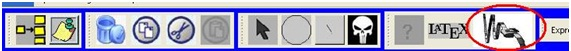
\includegraphics[width=\textwidth]{turi2.jpg}
\end{center}

Una vez pulsado el bot\'on, se abrir\'a el usual di\'alogo de apertura de archivos. Seleccionado el archivo, el algoritmo pasa a realizar los siguientes pasos:
\begin{enumerate}
\item Busca el primer estado para iniciar el procesamiento de la cinta (archivo de texto).
\item Coloca la cabeza lectora al principio de la cinta (primer s\'imbolo que no es un blanco).
\item Analiza que transici\'on entre las existentes en la m\'aquina, contienen el estado inicial y el car\'acter actual de la cabeza lectora.
\item Si existe la transici\'on, actualiza el valor de la celda de la cinta y se desplaza a la celda que indique la propia transici\'on (N =  no se desplaza, I = izquierda, D = derecha). Si no existe, la palabra no ser\'a reconocida, mostrando en el archivo de texto dicha situaci\'on.
\item Vuelve al paso 3 para ver si la nueva transici\'on existe (pero ahora con el estado y el s\'imbolo de cinta actualizados) y en caso afirmativo, tratarla de la misma manera, modificando la cinta.
\item Si al final de todo el c\'omputo, la palabra resulta reconocida, la salida que se ofrecer\'a en la cinta (archivo de texto) de la m\'aquina de Turing (por definici\'on) ser\'a la celda que se encuentra inmediatamente a la derecha de la \'ultima posici\'on de la cinta de entrada que no es un blanco de cinta.
\end{enumerate}

\subsection{Ampliaciones y problemas}
No hemos mencionado en la anterior descripci\'on del algoritmo, el caso en el que una m\'aquina de Turing, no acabe nunca su c\'omputo, es decir, cicle o no sea terminante.
Este problema no es decidible, ni siquiera existe una m\'aquina de Turing para esto.
Por ello recurrimos a una idea que si bien no ser\'a capaz de solucionar todos los casos, si un alto porcentaje de ellos.
Supongamos una m\'aquina de Turing y una palabra x dada, dicha m\'aquina puede:
\begin{itemize}
\item Aceptar a x, si existe una configuraci\'on de parada y aceptadora.
\item Rechazar a x, si existe una configuraci\'on de parada y no aceptadora.
\item Ciclar, si no existe una configuraci\'on de parada.
\end{itemize}
Dado que en un principio este problema no fue contemplado, era necesario a\~nadir alg\'un tipo de complemento para que se detectase el caso de ciclo en el c\'omputo de una m\'aquina de Turing. Dicho complemento, es una cota que utilizan varios algoritmos conocidos. Dicha cota est\'a relacionada con la longitud de la cinta y el n\'umero de transiciones de la m\'aquina de Turing  y su tratamiento consiste en consultar el n\'umero de transiciones visitadas hasta el momento y compararlas con dicha cota.



\section{Cambios destacables en TALFi 2.0}
\subsection{Interfaz gr\'afica}
Ante todo hemos de decir que nuestro objetivo ha sido incluir las nuevas funciones de TALFi alterando lo m\'inimo posible el dise\~no que hasta el momento ten\'ia la aplicaci\'on.\\

{\bf Notaci\'on gr\'afica para autom\'atas de pila\\}

Un diagrama que generaliza el diagrama de transici\'on de un aut\'omata finito
aclara determinados aspectos del comportamiento de un aut\'omata de pila. Por lo
tanto, introduciremos y usaremos a partir de ahora un diagrama de transici\'on para
aut\'omatas de pila en el que:
\begin{enumerate}
\item Los nodos corresponden a los estados del aut\'omata de pila.
\item Una tri\'angulo blanco indica el estado inicial, y los estados con un doble c\'irculo
son de aceptaci\'on, igual que en la primera versi\'on de TALFi cuando se dibujan los
aut\'omatas finitos.
\item Los arcos corresponden a las transiciones del aut\'omata de pila en el sentido
siguiente:\\ un arco con la etiqueta a/X/$\alpha$ desde el estado q al estado p significa
que $\delta$(q,a,X) contiene el par (p,$\alpha$), quiz\'a entre otros pares. Es decir, la
etiqueta del arco dice qu\'e entrada se usa y tambi\'en indica los elementos de lo alto
de la pila, antiguo y nuevos.
La \'unica cosa que el diagrama no nos dice es qu\'e s\'imbolo de la pila es el s\'imbolo
inicial. Por convenio, ser\'a $Z_{0}$, a menos que se tenga que transformar un
aut\'omata de pila que acepte un lenguaje por estado final en otro que acepte el mismo
lenguaje por pila vac\'ia, siendo en ese caso $X_{0}$.\\
\end{enumerate}
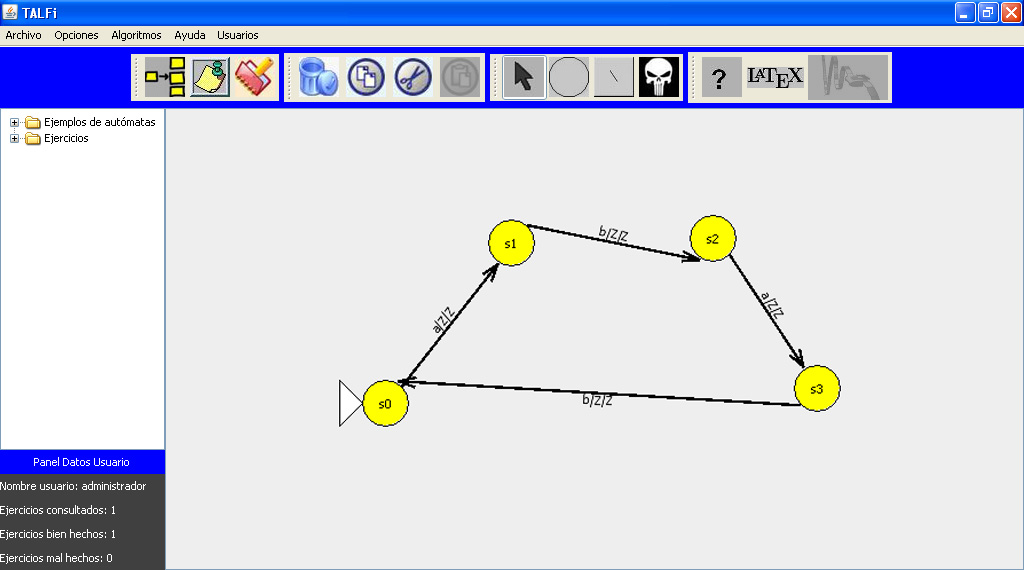
\includegraphics[width=\textwidth]{graficoaristasparapila.jpg} \\
{\bf Notaci\'on gr\'afica para m\'aquinas de Turing\\}


Las transiciones de una m\'aquina de Turing pueden representarse visualmente de
una forma muy parecida como se hace para los aut\'omatas de pila. Un diagrama de
transici\'on est\'a formado por un conjunto de nodos que corresponden a los estados
de la m\'aquina de Turing. En un arco que vaya del estado q al estado p, aparecer\'an
una o varias etiquetas de la forma X/Y/S, d\'onde X e Y son s\'imbolos de cinta, y S
indica un sentido, que puede der I, D o N. Es decir, si $\delta$(q,X) = (p,Y,S), en el
arco que va de q a p se encontrar\'a la etiqueta X/Y/S.
Como en el resto de diagramas de transici\'on, el estado inicial se indica mediante la
colocaci\'on de un tri\'angulo blanco a su izquierda, y los estados se aceptaci\'on se
indican mediante c\'irculos dobles.

Por tanto, la \'unica informaci\'on sobre la m\'aquina
de Turing que habr\'ia que a\~nadir al diagrama es el s\'imbolo que se utiliza para
denotar el espacio en blanco. Dicho s\'imbolo es \#. \\
\begin{center}
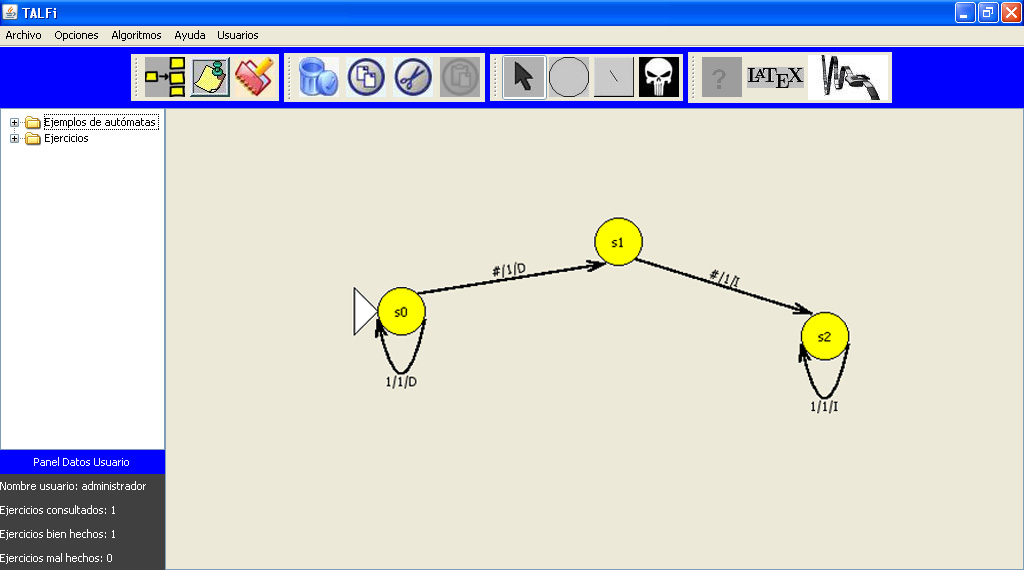
\includegraphics[width=\textwidth]{graficoaristasparaturing.jpg} \\
\end{center}



{\bf Crear un nuevo aut\'omata de pila / m\'aquina de Turing\\}

Para no saturar m\'as de botones, no hemos incluido uno que fuera un acceso directo para crear un nuevo ejemplo de m\'aquina de Turing o aut\'omata de pila. Si el usuario desea un nuevo ejemplo de estas caracter\'isticas, tendr\'a que dirigirse y hacer click en el apartado ``Archivo'' del men\'u superior:\\
\begin{center}
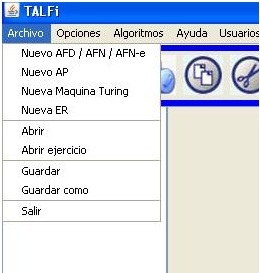
\includegraphics[width=\textwidth]{roci2.jpg}
\end{center}
{\bf  Botones\\}

La segunda novedad son los tres botones para la generaci\'on aleatoria de palabras para aut\'omatas de pila, cargar la cinta inicial de la m\'aquina de Turing y la generaci\'on del c\'odigo en \LaTeX{} del aut\'omata que visualizamos en el canvas.\\
\newline
Al comienzo de la aplicaci\'on aparecen los tres desactivados, y seg\'un las \'areas que trabajemos se ir\'an activando si corresponde.\\ Lo mismo ocurre con la secci\'on algoritmos, las opciones est\'an \'unicamente disponibles cuando sea l\'ogico el poder aplicarlas.\newline

Aspecto de la aplicaci\'on al arrancarla:\\
\begin{center}
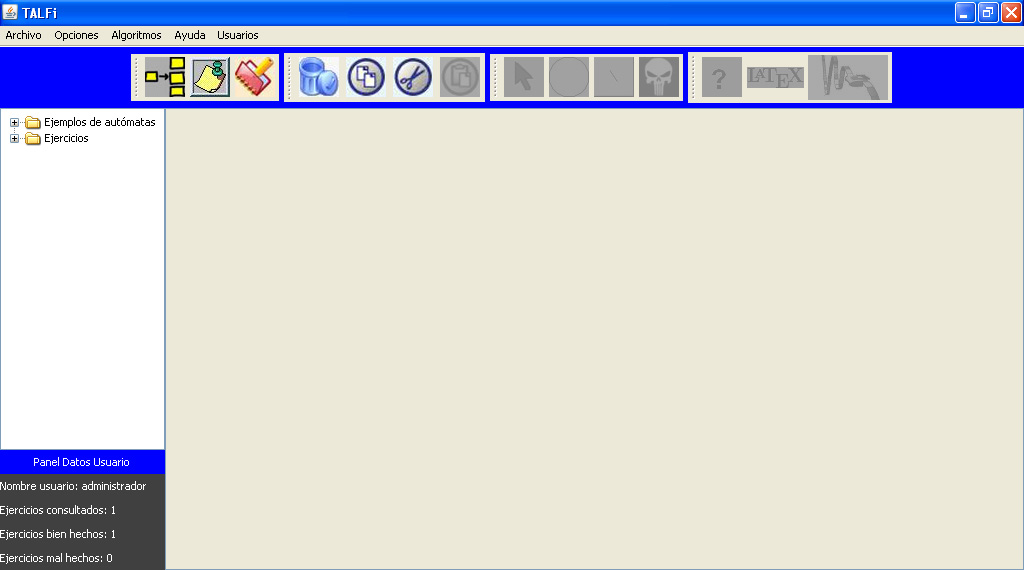
\includegraphics[width=\textwidth]{inicial.jpg}
\end{center}

\newpage

Men\'u Algoritmos al iniciar la aplicaci\'on:\\
\begin{center}
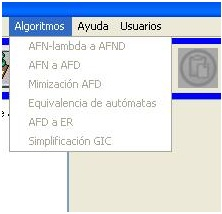
\includegraphics[width=\textwidth]{roci4.jpg}
\end{center}
Muestra de los botones activos en un ejemplo de m\'aquina de Turing:\\
\begin{center}
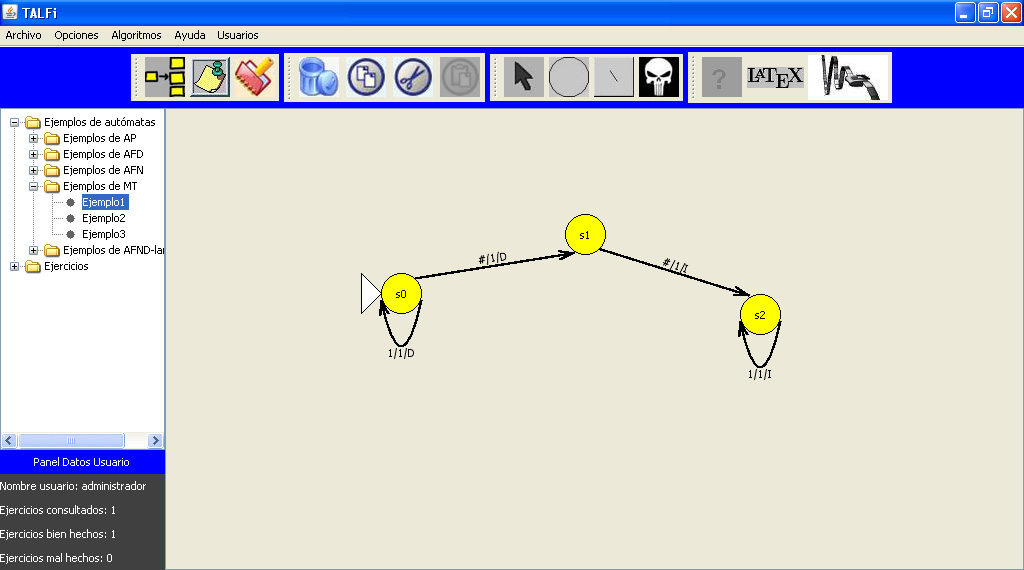
\includegraphics[width=\textwidth]{roci52.jpg}
\end{center}



\newpage
Cuadro de di\'{a}logo que aparece al modificar una arista de un aut\'omata de pila:\\
\begin{center}
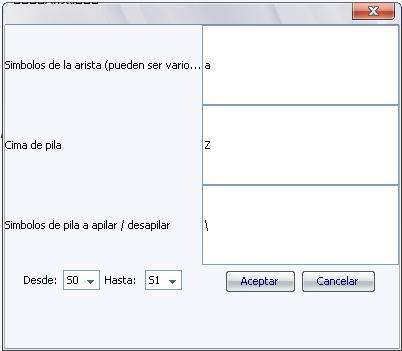
\includegraphics[scale=0.6]{roci6.jpg}
\end{center}



\subsection{Ejercicios\\}
Ahora tambi\'en es posible crear ejercicios de aut\'omatas de pila y m\'aquinas de Turing. Hemos incluido una peque\~na colecci\'on, pero el administrador puede ampliarla creando sus propios ejercicios y a\~nadi\'endolos a la base de datos de los mismos. A continuaci\'on detallaremos como crearlos, que informaci\'on interna generan, y la forma de corregirlos que hemos implementado.\\
Se siguen creando de la misma manera que los anteriores ejercicios,\\ seleccion\'andolos de la lista de todos los posibles:
\begin{center}
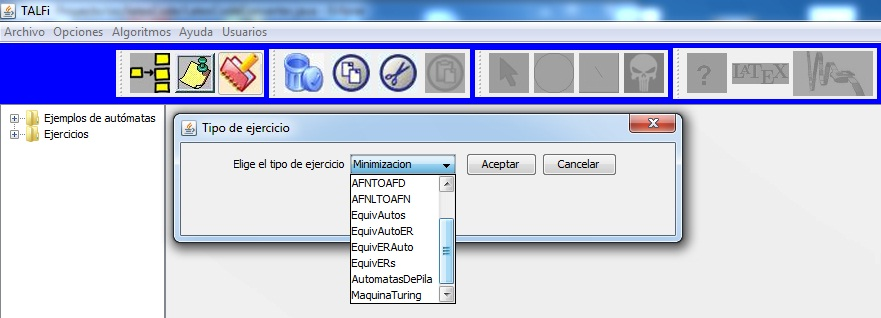
\includegraphics[width=\textwidth]{ejer1.jpg}
\end{center}

Hasta el momento, el administrador solamente ten\'ia que dibujar el aut\'o-\\mata o escribir la expresi\'on regular que fuera soluci\'on, y el enunciado del ejercicio. Para los nuevos ejercicios necesitamos m\'as informaci\'on para poder asegurar que la soluci\'on que proporcione el usuario es la suministrada por el administrador de la aplicaci\'on. A continuaci\'on describimos los cambios introducidos.\\

{\bf Interfaz gr\'{a}fica  para ejercicios de aut\'{o}matas de pila \\}

Un lenguaje independiente de contexto puede generarse con distintas gram\'aticas independientes de contexto, y por tanto con diferentes aut\'omatas de pila. Por este motivo, necesitamos tener una lista de palabras que tendremos que comprobar que son aceptadas el aut\'omata de pila dibujado como soluci\'on, resultado que obtenemos f\'acilmente mediante el resultado que obtenemos al aplicar el algoritmo CYK. Para afinar m\'as a\'un el resultado, pedimos otra lista de palabras que no deben ser reconocidas por el a\'utomata. Ninguna de las dos tiene l\'imite, pero si es necesario que alguna de ellas contenga alguna cadena, pues con ambas vac\'ias no podr\'iamos comparar la soluci\'on del ejercicio con la que nos proporcione el usuario.

\begin{center}
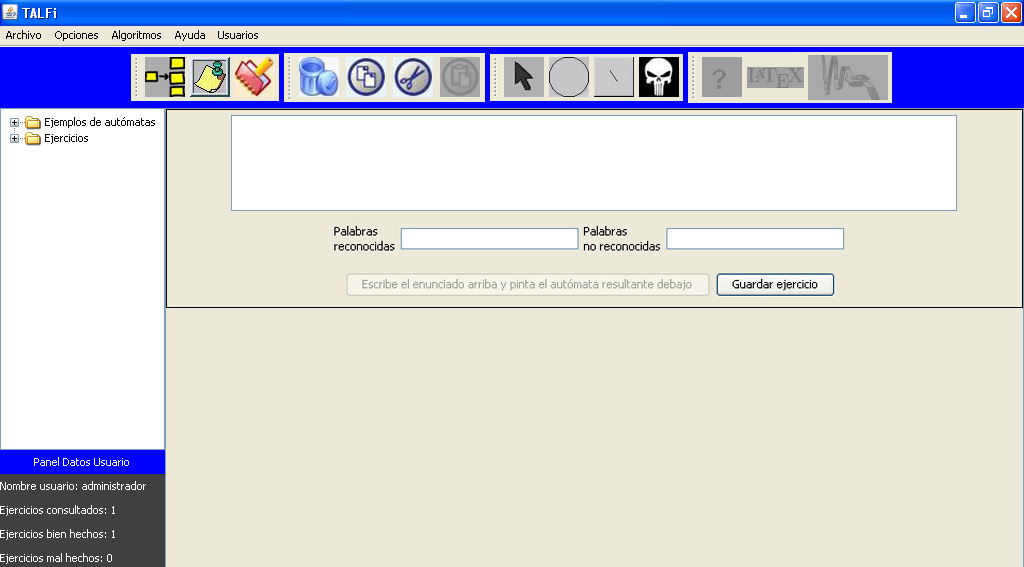
\includegraphics[width=\textwidth]{crearejpila.jpg}
\end{center}
Al aut\'omata que pinte el usuario se le aplicar\'a el algoritmo de CYK, y si coinciden todos los resultados, se considerar\'a el ejercicio como apto, en otro caso no se dar\'a como no v\'alido.\\
\newline \newline \newline \newline \newline
El usuario que vaya a enviar la correci\'on del ejercicio en ning\'un momento tendr\'a conocimiento de cuales son las palabras que pertenecen a estas listas.\\

{\bf Simulaci\'{o}n de la correci\'{o}n del ejercicio 4 de la colecci\'{o}n de ejercicios de aut\'{o}matas de pila de TALFi}

\begin{center}
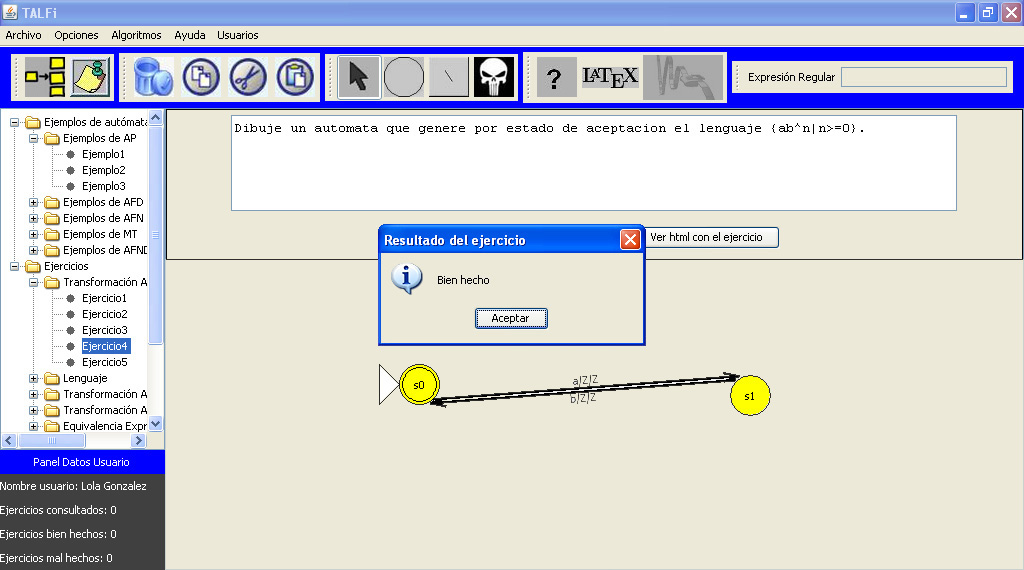
\includegraphics[width=\textwidth]{resolucionej4.jpg}
\end{center} 

{\bf  Interfaz gr\'{a}fica para ejercicios de m\'aquinas de Turing \\}

La correci\'on de ejercicios depender\'a de si la soluci\'on tiene estados finales o no, puesto que en el primer caso, en los c\'omputos que finalizan no nos importa el contenido de la cinta, pero sin embargo en el segundo s\'i. Como no sabemos si se va a crear un ejercicio cuya soluci\'on tenga estados finales, incluimos cinco casillas, en las cu\'ales se podr\'an escribir las cintas de entrada que ser\'an aceptadas, las salidas de cinta generadas por las cintas de entrada aceptadas, las cintas de entrada que no ser\'an aceptadas, las salidas de cinta generadas por las cintas de entrada que no se aceptar\'an, y las cintas de entrada que provocar\'an ciclos en la simulaci\'on.  No es necesario rellenar toda esta informaci\'on, pero si alguno, pues sino es imposible corregir el ejercicio.


\begin{center}
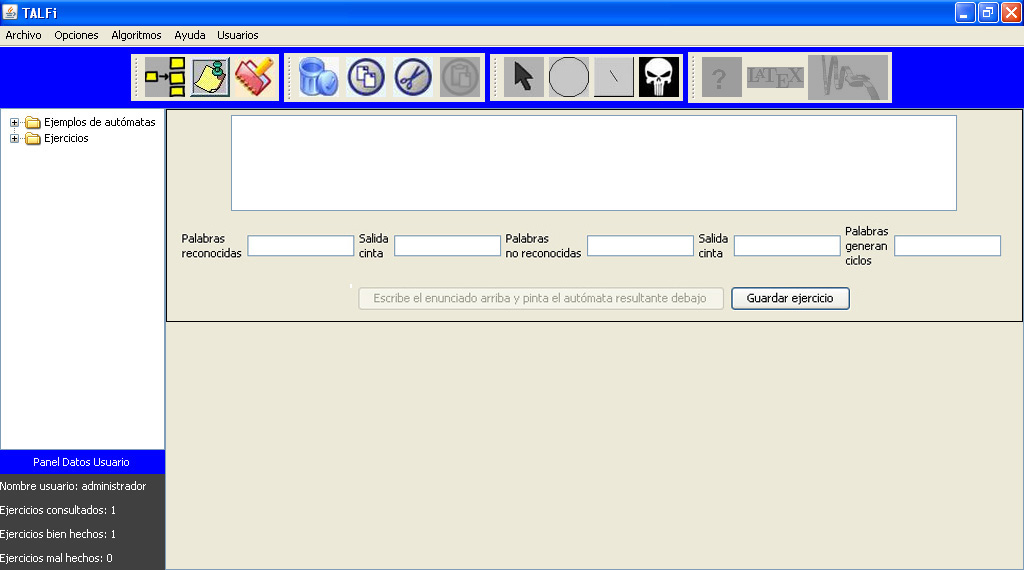
\includegraphics[width=\textwidth]{crearejmt.jpg}
\end{center} 

Si la soluci\'on del ejercicio no contiene estados finales, comprobaremos que las cintas de entrada con sus cintas de salidas asociadas contienen el mismo n\'umero de elementos. Si son distintos avisamos al administrador para que las revise.\\
No se generar\'an las cintas de salida obtenidas en el caso de que pare la simulaci\'on, ya que s\'olo necesitamos saber si se ha obtenido la misma salida en la soluci\'on que en la simulaci\'on de la respuesta dibujada por el usuario.


\chapter{Entorno \LaTeX{}}
\section{\LaTeX{}}

La opci\'on de que TALFi imprimiese cualquier aut\'omata que se dibujase en {\LaTeX{}} o mostrase los pasos de una simplificaci\'on de gram\'aticas en dicho formato, no fue uno de los riquisitos de la especificaci\'on en un principio.\\
Pero la opci\'on concedida gracias a una beca del PIE (Programa de Iniciaci\'on a la Empresa), nos dio la oportunidad de a\~nadir esta funcionalidad a la aplicaci\'on y poder trabajar con este formato de texto tan usado entre profesionales.\\
\subsection{Introducc\'on a \LaTeX{}}
\LaTeX{} es un sistema de composici\'on de textos, orientado especialmente a la creaci\'on de libros, documentos cient\'ificos y t\'ecnicos que contengan f\'ormulas matem\'aticas.

\LaTeX{} est\'a formado por un gran conjunto de macros de \TeX{}, escrito por Leslie Lamport en 1984, con la intenci\'on de facilitar el uso del lenguaje de composici\'on tipogr\'afica \TeX{}, creado por Donald Knuth. Es muy utilizado para la composici\'on de art\'iculos acad\'emicos, tesis y libros t\'ecnicos, dado que la calidad tipogr\'afica de los documentos realizados con \LaTeX{} es comparable a la de una editorial cient\'ifica de primera l\'inea.

\LaTeX{} es software libre bajo licencia LPPL.


\subsection{Descripci\'on:}
\LaTeX{} es un sistema de composici\'on de textos que est\'a formado mayoritariamente por \'ordenes (macros) construidas a partir de comandos de \TeX{} ---un lenguaje ``de bajo nivel'', en el sentido de que sus acciones \'ultimas son muy elementales--- pero con la ventaja a\~nadida, en palabras de Lamport, de ``poder aumentar las capacidades de \LaTeX{} utilizando comandos propios del \TeX{} descritos en The TeXbook''. Esto es lo que convierte a \LaTeX{} en una herramienta pr\'actica y \'util pues, a su facilidad de uso, se une toda la potencia de \TeX{}. Estas caracter\'isticas hicieron que \LaTeX{} se extendiese r\'apidamente entre un amplio sector cient\'ifico y t\'ecnico, hasta el punto de convertirse en uso obligado en comunicaciones y congresos, y requerido por determinadas revistas a la hora de entregar art\'iculos acad\'emicos.

Su c\'odigo abierto permiti\'o que muchos usuarios realizasen nuevas utilidades que extendiesen sus capacidades con objetivos muy variados, a veces ajenos a la intenci\'on con la que fue creado: aparecieron diferentes dialectos de \LaTeX{} que, a veces, eran incompatibles entre s\'i. Para atajar este problema, en 1989 Lamport y otros desarrolladores iniciaron el llamado ``Proyecto LaTeX3''. En oto\~no de 1993 se anunci\'o una reestandarizaci\'on completa de \LaTeX{}, mediante una nueva versi\'on que inclu\'ia la mayor parte de estas extensiones adicionales (como la opci\'on para escribir transparencias o la simbolog\'ia de la American Mathematical Society) con el objetivo de dar uniformidad al conjunto y evitar la fragmentaci\'on entre versiones incompatibles de \LaTeX{} 2.09. Esta tarea la realizaron Frank Mittlebach, Johannes Braams, Chris Rowley y Sebastian Rahtz junto al propio Leslie Lamport. Hasta alcanzar el objetivo final del ``Proyecto 3'', a las distintas versiones se las viene denominando \LaTeX{}$2_\epsilon$ (o sea, ``versi\'on 2 y un poco m\'as...''). Actualmente cada a\~no se ofrece una nueva versi\'on, aunque las diferencias entre una y otra suelen ser muy peque\~nas y siempre bien documentadas.


Con todo, adem\'as de todas las nuevas extensiones, la caracter\'istica m\'as relevante de este esfuerzo de reestandarizaci\'on fue la arquitectura modular: se estableci\'o un n\'ucleo central (el compilador) que mantiene las funcionalidades de la versi\'on anterior pero permite incrementar su potencia y versatilidad por medio de diferentes paquetes que solo se cargan si son necesarios. De ese modo, \LaTeX{} dispone ahora de innumerables paquetes para todo tipo de objetivos, muchos dentro de la distribuci\'on oficial, y otros realizados por terceros, en algunos casos para usos especializados.

\section{Uso}
\LaTeX{} presupone una filosof\'ia de trabajo diferente a la de los procesadores de texto habituales (conocidos como WYSIWYG, es decir, ``lo que ves es lo que obtienes'') y se basa en comandos. Tradicionalmente, este aspecto se ha considerado una desventaja (probablemente la \'unica). Sin embargo, \LaTeX{}, a diferencia de los procesadores de texto de tipo WYSIWYG, permite a quien escribe un documento centrarse exclusivamente en el contenido, sin tener que preocuparse de los detalles del formato. Adem\'as de sus capacidades gr\'aficas para representar ecuaciones, f\'ormulas complicadas, notaci\'on cient\'ifica e incluso musical, permite estructurar f\'acilmente el documento (con cap\'itulos, secciones, notas, bibliograf\'ia, \'indices anal\'iticos, etc.), lo cual brinda comodidad y lo hace \'util para art\'iculos acad\'emicos y libros t\'ecnicos.\\

Con \LaTeX{}, la elaboraci\'on del documento requiere normalmente de dos etapas: en la primera hay que crear mediante cualquier editor de texto llano un fichero fuente que, con las \'ordenes y comandos adecuados, contenga el texto que queramos imprimir. La segunda consiste en procesar este fichero; el procesador de textos interpreta las \'ordenes escritas en \'el y compila el documento, dej\'andolo preparado para que pueda ser enviado a la salida correspondiente, ya sea la pantalla o la impresora. Ahora bien, si se quiere a\~nadir o cambiar algo en el documento, se deber\'a hacer los cambios en el fichero fuente y procesarlo de nuevo. Esta idea, que puede parecer poco pr\'actica a priori, es conocida a los que est\'an familiarizados con el proceso de compilaci\'on que se realiza con los lenguajes de programaci\'on de alto nivel (C, C++, etc.), ya que es completamente an\'alogo.\\

El modo en que \LaTeX{} interpreta la ``forma'' que debe tener el documento es mediante etiquetas. Por ejemplo, ``documentclass\{article\}'' le dice a \LaTeX{} que el documento que va a procesar es un art\'iculo. Puede resultar extra\~no que hoy en d\'ia se siga usando algo que no es WYSIWYG, pero las caracter\'isticas de \LaTeX{} siguen siendo muchas y muy variadas. Tambi\'en hay varias herramientas (aplicaciones) que ayudan a una persona a escribir estos documentos de una manera m\'as visual (LyX, TeXmacs y otros). A estas herramientas se les llama WYSIWYM (``lo que ves es lo que quieres decir'').\\

Una de las ventajas de \LaTeX{} es que la salida que ofrece es siempre la misma, con independencia del dispositivo (impresora, pantalla, etc.) o el sistema operativo (MS Windows, MacOS, Unix, GNU/Linux, etc.) y puede ser exportado a partir de una misma fuente a numerosos formatos tales como Postscript, PDF, SGML, HTML, RTF, etc. Existen distribuciones e IDEs de LaTeX para todos los sistemas operativos m\'as extendidos, que incluyen todo lo necesario para trabajar. Hay, por ejemplo, programas para Windows como TeXnicCenter, \htmladdnormallink{MikTeX}{http://miktex.org/} o \htmladdnormallink{WinEdt}{http://www.winedt.com/}, para Linux como Kile, o para MacOS como TeXShop, todos liberados bajo la Licencia GPL. Existe adem\'as un editor multiplataforma (para MacOS, Windows y Unix) llamado Texmaker, que tambi\'en tiene licencia \htmladdnormallink{GPL}{http://es.wikipedia.org/wiki/Licencia_publica_general_de_GNU}.

\subsection{Uso de \LaTeX en la herramienta TALFi\\}
Aunque \LaTeX es primordialmente un sistema de composici\'on de textos para la creaci\'on de documentos que contengan f\'ormulas matem\'aticas, en TALFi lo usaremos para poder colocar en nuestros textos aut\'omatas o simplificaciones paso a paso de gram\'aticas. 

Esto es posible debido a una gran cantidad y diversidad de bibliotecas/paquetes que podemos a\~nadir a nuestro editor de \LaTeX{}.
Gracias a esta amplitud de posibilidades para crear gr\'aficos complejos en \LaTeX{}, el trabajo inicial de poder imprimir los aut\'omatas o las simplificaciones acab\'o dando como resultado 3 posibles representaciones en \LaTeX{}. De esta manera y debido a las diferencias entre las representaciones, el usuario podr\'a elegir entre un dise\~no sobrio y con formas claras, un dise\~no colorido o un dise\~no en forma matricial para poder modificarlo de manera m\'as intuitiva.

Sin embargo para la representaci\'on de los pasos en la simplificaci\'on de gram\'aticas, s\'olo disponemos de un dise\~no, puesto que la representaci\'on se hace mediante tablas y texto plano, siendo innecesaria la inclusi\'on de colores, formas, etc.

\section{LatexCodeConverter\\}
Esta clase, es la encargada de traducir cualquier aut\'omata de TALFi en un archivo \TeX{} totalmente listo para ser compilado en cualquier entorno para \LaTeX{}.
\newline
\begin{itemize}
\item Algoritmo conversor:\\
\newline
La implementaci\'on del algoritmo consiste b\'asicamente en traducir los distintos campos de los que consta un aut\'omata en comandos \LaTeX{}:
\begin{enumerate}
\item Para cada estado del aut\'omata se crea un c\'irculo en el que dentro se incluye su etiqueta. Se detectan el estado inicial y los de aceptaci\'on, para los que se usan otra representaci\'on, adem\'as de su c\'irculo.
\item Se toma cada coordenada de cada nodo del aut\'omata TALFi para colocarlo de la misma manera en el archivo que generemos con \LaTeX{}.
\item Generamos las aristas viendo desde que estado parten y a cual se dirigen.
\item Cerramos el archivo.\\
\end{enumerate}

\item Representaciones:\\
\begin{enumerate}
\item Mediante biblioteca xy:\\
\newline
Esta es la representaci\'on m\'as fiable y visualmente m\'as clara, puesto que siempre que se pueda dibujar un aut\'omata en TALFi, su representaci\'on en \LaTeX ser\'a pr\'acticamente id\'entica.\\
\begin{center}
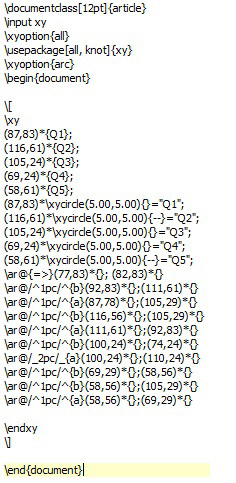
\includegraphics{lateaux.jpg}
\end{center}
\begin{center}
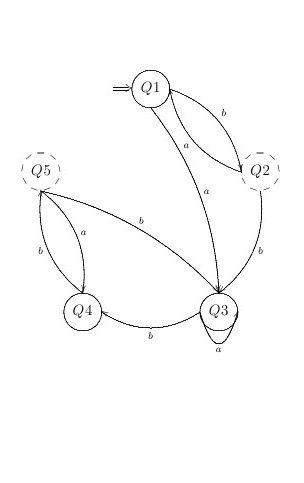
\includegraphics{lateaux2.jpg}
\end{center}


\item Mediante biblioteca TikZ:\\
\newline
Esta biblioteca es visualmente muy atractiva, pero tiene el incoveniente de que el modo en el que los estados se colocan en el lienzo, se realiza especificando donde se encuentran cada uno de ellos, en relaci\'on a un estado dado.
Como vemos en el c\'odigo, partimos del estado A ($q_{a}$ en el dibujo), para luego indicar que el estado B se encuentra arriba y a la derecha del estado A. Lo mismo ocurre con el estado C, que se indica que est\'a abajo y a la derecha del estado B,etc.\\
\newline
Aunque visualmente gane muchos enteros este tipo de representaci\'on, debido a que el algoritmo construye el dibujo de manera de autom\'atica, puede llevar a muchos problemas de superposici\'on de estados cuando los aut\'omatas contienen un n\'umero de estados elevado (inlcuso pord\'ia no poder visualizarse).\\ 
Conllevar\'ia una trabajo dificultoso de grafos para llevar a cabo una representaci\'on de aut\'omatas totalmente libre de errores para esta representaci\'on.
No obstante, si se quieren incluir aut\'omatas en un texto \LaTeX{} de manera manual, este es el mejor m\'etodo posible.\\

Lo comprobamos en un ejemplo:\newline \newline
\begin{center}
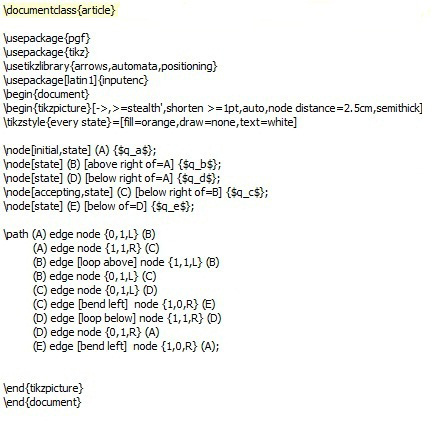
\includegraphics{late2aux.jpg}
\end{center}

\newpage

\begin{center}
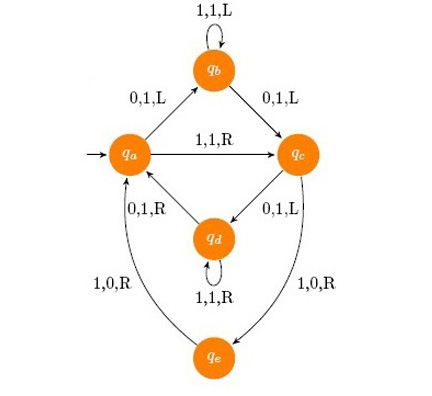
\includegraphics{late2aux2.jpg}
\end{center}

\item Mediante biblioteca Psmatrix:\\
\newline
En esta implementaci\'on, no cabe posibilidad de solapamiento de estados, puesto que cada uno ocupar\'a una ``celda'' de una matriz virtual que se crea en el lienzo.\\
Sin embargo, al igual que ocurr\'ia en el caso anterior, ante aut\'omatas con gran cantidad de estados, nos vamos a encontrar con un problema.\\
\newline
En este caso el problema, ser\'a visual. Puesto que al haber tal cantidad de estados y debido a su disposici\'on matricial, las numerosas aristas, pasar\'an por el centro de la matriz con toda seguridad, no permitiendo observar bien las etiquetas de las transiciones e incluso no pudiendo ver desde donde o hacia donde se dirigen.

\end{enumerate}
\end{itemize} 
\begin{center}
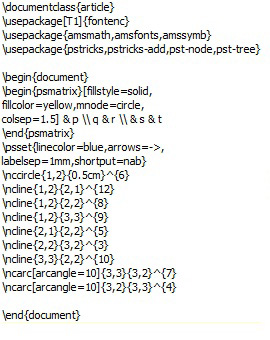
\includegraphics{latee1.jpg}
\end{center}

\begin{center}
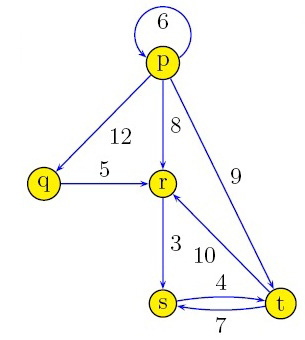
\includegraphics{latee2.jpg}
\end{center}

\section{TraductorHTML}

En TALFi 1.0 esta clase se encargaba de mostrar un archivo HTML en un navegador web, con los pasos de la minimizaci\'on de aut\'omatas finitos.\\
\newline
Ahora se ha ampliado su funcionalidad para que muestre tambi\'en la simplificaci\'on de gram\'aticas y la anteriormente mencionada minimizaci\'on, en \LaTeX{}.\\
\newline
Para ello usamos los comandos \LaTeX{} $\bf{tabular}$ y $\bf{hline}$ para dar un formato parecido a las tablas que se generebana en html. De esta manera podemos crear l\'ineas verticales y horizontales para dar aspecto de tabla en \LaTeX{}.\\
\newline
El resto es introducir texto plano y los atributos de las distintas gram\'aticas que se van simplificando.\newline

\begin{center}
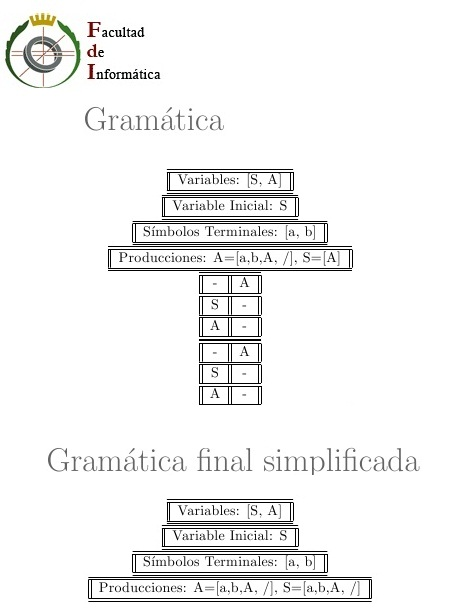
\includegraphics[scale=0.7]{late3.jpg}
\end{center}

\newpage
\section{Entornos \LaTeX{} utilizados}
\begin{itemize}
\item Miktex:
\begin{center}
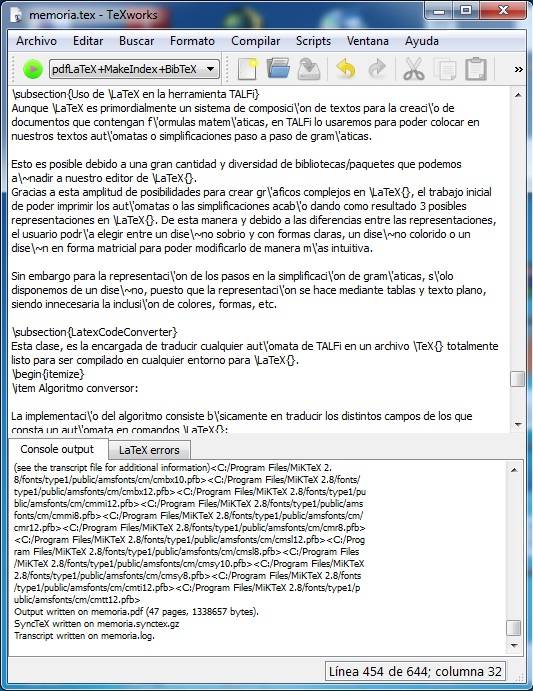
\includegraphics[scale=0.7]{prog1.jpg}
\end{center}
MiKTeX es una distribuci\'on \TeX{}/\LaTeX{} para Microsoft Windows que fue desarrollada por Christian Schenk.
Las caracter\'isticas m\'as apreciables de MiKTeX son su habilidad de actualizarse por s\'i mismo descargando nuevas versiones de componentes y paquetes instalados previamente, y su f\'acil proceso de instalaci\'on.\\
La versi\'on actual de MiKTeX es 2.8 y est\'a disponible en su \htmladdnormallink{p\'agina oficial}{http://miktex.org/}. Adem\'as, tiene caracter\'isticas que incluyen MetaPost y pdfTeX y compatibilidad con Windows 7. A partir de la versi\'on 2.7 se incluy\'o soporte integrado para XeTeX.
\newline \newline \newline \newline

Caracter\'isticas:
\begin{itemize}
\item Es libre y f\'acil de instalar.
\item Incluye m\'as de 800 paquetes con fonts, macros, etc.
\item Tiene un visor propio de archivos dvi denominado Yap.
\item Su c\'odigo es abierto.
\item Posee compiladores \TeX{} y \LaTeX{}, convertidores para generar archivos postscripts (.ps), pdf , html , etc.; y herramientas para generar bibliograf\'ias e \'indices.
\item Posee tres formas de instalaci\'on: peque\~na, mediana y completa.
\end{itemize}

\item WinEdt:
\begin{center}
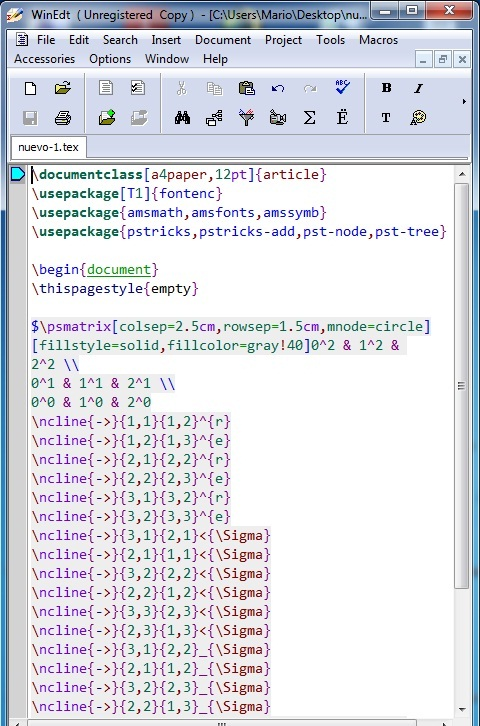
\includegraphics[scale=0.7]{prog2.jpg}
\end{center}
WinEdt es un editor de textos de gran alcance y versatilidad para Windows, con una fuerte predisposici\'on hacia la creaci\'on de documentos \LaTeX{}. 
La \htmladdnormallink{p\'agina de descargas}{http://www.winedt.com/index.html} del sitio web  tiene m\'as informaci\'on sobre WinEdt, \TeX{}, y enlaces a otros programas necesarios para hacer operativo WinEdt en la plataforma Windows.
\end{itemize}

\clearemptydoublepage
\chapter{Anexos}
\section{Ampliaci\'on del Manual de Usuario}
Antes de que cualquier persona, administrador o no, quiera usar TALFi 2.0, debe conocer dos detalles para poder usar la aplicaci\'on correctamente:\\
\begin{itemize}
\item Si quiere incluir $\epsilon$ en las transiciones, tendr\'a que hacerlo de forma distinta que en TALFi 1.0, con el car\'acter \verb'\'.
\item Por defecto el s\'imbolo de fondo de pila es Z.
\item Para especificar un blanco en m\'aquinas de Turing, tendr\'a que escribir $\#$.
\item Las direcciones posibles de movimiento en m\'aquinas de Turing son I, D, N para espa\~nol, y L,R,N para ingl\'es. Ambas siempre en may\'usculas. 
\item Necesariamente el contenido de la cinta para simular una m\'aquina de Turing debe cargarse en un archivo con extensi\'on ``txt''.
\item Los enunciados de los ejercicios no pueden contener acentos ni el car\'acter `\~{n}'.
\item Para especificar una cinta de blancos en los ejercicios de m\'aquinas de Turing, tendr\'a que escribir $\#$.
\end{itemize}
Al igual que en la primera versi\'on de TALFi, cuando se pide introducir los s\'imbolos, ya sean de cinta o de alfabeto, en ning\'un caso deben contener espacios y tienen que ir separados por comas.


\section{Cambios en la implementaci\'on}
A continuaci\'on enumeraremos brevemente las nuevas clases y los nuevos paquetes creados en este proyecto.\\
\newline
{\bf Ampliaci\'{o}n de paquetes}

\begin{itemize}
\item Modelo.algoritmos:

\begin{itemize}
\item AceptaTuring:\\Contiene el algoritmo que simular\'ia la ejecuci\'on de una m\'aquina de Turing. Recibe el objeto creado para m\'aquinas de Turing y la ruta del archivo que contiene la cinta. Aqu\'i se abre, si ocurriese alg\'un problema no se realiza la simulaci\'on.
\item AutomataP\_to\_GramaticaIC:\\Dado un aut\'omata de pila aplicamos el algoritmo que nos genera su gram\'atica asociada.
\item GIC\_to\_FNC:\\Recibe la gram\'atica que ha generado AutomataP\_to\_GramaticaIC, y la transforma en Forma Normal de Greibach con el algoritmo que utiliza las tablas de reemplazo.
\item GIC\_to\_Chomsky:\\Al igual que GIC\_to\_FNC, genera la correspondiente Forma Normal de Chomsky a partir de la gram\'atica obtenida en AutomataP\_to\_GramaticaIC.
\item C\_Y\_K:\\ Implementa el algoritmo CYK y guarda la lista de palabras que van a ejecutarse sobre \'el, al igual que la salida que generan, y sobre qu\'e gram\'atica independiente de contexto lo hacen.
\item TuringResultado:\\Contiene la m\'aquina de Turing a corregir junto con la informaci\'on necesaria para ello y la lista de resultados que se obtienen.

\end{itemize}
\item Modelo.automatas:
\begin{itemize}
\item Alfabeto\_Pila: \\Interface con las operaciones de alfabetos de pila.
\item AlfabetoPila\_imp:\\Implementa Alfabeto\_Pila y es la clase que como su nombre indica crea y contiene informaci\'on del alfabeto de pila.
\item AlfabetoCinta:\\Crea el alfabeto de cinta de una m\'aquina de Turing.
\item AutomataPila:\\Sirve para crear objetos que identifiquen aut\'omatas de pila.
\item MaquinaTuring:\\Sirve para crear objetos que identifiquen m\'aquinas de Turing.
\end{itemize}
\item Vista.vistaGrafica:
\begin{itemize}
\item AristaGeneral:\\Clase abstracta con todos los atributos y m\'etodos comunes a todos los tipos de aristas.
\item Arista:\\Arista utilizada para todos los aut\'omatas finitos.
\item AristaAP:\\Arista que se utiliza en aut\'omatas de pila.
\item AristaTuring:\\Arista que se emplea en m\'aquinas de Turing.\\
\end{itemize}
\item Vista.vistaGrafica.events:
\begin{itemize}
\item OyenteItemPopupAristaAP:\\Crea el cuadro de di\'alogo cuando se modifica una arista de un aut\'omata de pila.
\item OyenteItemPopupAristaTuring:\\Crea el cuadro de di\'alogo cuando se modifica una arista de una m\'aquina de Turing.
\item OyenteModificaAristaAPActionListener:\\Procesa los nuevos atributos que se han cambiado al modificar la arista de un aut\'omata de pila si se pulsa aceptar con el rat\'on.
\item OyenteModificaAristaTuringActionListener:\\Procesa los nuevos atributos que se han cambiado al modificar la arista de una m\'aquina de Turing si se pulsa aceptar con el rat\'on.
\item OyenteModificaAristaAPKeyAdapter:\\Procesa los nuevos atributos que se han cambiado al modificar la arista de un aut\'omata de pila si se aceptan pulsando Intro.
\item OyenteModificaAristaTuringKeyAdapter:\\Procesa los nuevos atributos que se han cambiado al modificar la arista de una m\'aquina de Turing si se aceptan pulsando Intro.
\end{itemize}
\end{itemize}

{\bf Creaci\'{o}n de paquetes:}
\begin{itemize}
\item Modelo.gramatica:\\
\begin{itemize}
\item Chomsky:\\Crea objetos que representen una gram\'atica en Forma Normal de Chomsky.
\item Gramatica:\\Clase abstracta con los atributos y m\'etodos comunes a todas las gram\'aticas que generamos en esta aplicaci\'on.
\item GramaticaIC:\\Clase que extiende a Gramatica, y cuyos objetos representan la gram\'atica resultante antes de transformarla en ninguna Forma Normal.
\item Greibach:\\Crea objetos que representen una gram\'atica en Forma Normal de Greibach.
\item Produccion:\\Crea los objetos que procesaremos como producciones.
\end{itemize}
\end{itemize}

\section{Estructura XML de los ejercicios de aut\'omatas de pila}
Incluimos la estructura interna de los ejercicios de aut\'omatas de pila, donde se apreciar la similitud con los ejercicios de la primera versi\'on de TALFi y las novedades incluidas en su ampliaci\'on.\\

{\ttfamily

\noindent$<$ejercicio$>$\\

$<$tipo$>$TransformacionAPs$<$/tipo$>$\\

$<$enunciado$>$\\

Dibuje un automata que genere por estado de aceptacion el lenguaje \{ab\char94n $|$ n$>$=0\}.\\

$<$/enunciado$>$\\

$<$output$>$\\

$<$authomata$>$\\

\indent $<$type$>$\\

\indent \indent $<$item$>$AutomataPila$<$/item$>$\\

\indent $<$/type$>$\\

\indent $<$alphabet$>$\\

\indent \indent $<$item$>$a$<$/item$>$\\

\indent \indent $<$item$>$b$<$/item$>$\\

\indent $<$/alphabet$>$\\

\indent \indent $<$alphabetP$>$\\

\indent \indent \indent $<$item$>$Z$<$/item$>$\\

\indent \indent $<$/alphabetP$>$\\

\indent $<$states$>$\\

\indent \indent $<$state$>$s2$<$/state$>$\\

\indent \indent $<$state$>$s1$<$/state$>$\\

\indent $<$/states$>$\\

\indent $<$init$>$\\

\indent \indent $<$state$>$s1$<$/state$>$\\

\indent $<$/init$>$\\

\indent $<$finals$>$\\

\indent \indent $<$state$>$s1$<$/state$>$\\

\indent $<$/finals$>$\\

\indent $<$arrows$>$\\

\indent \indent $<$arrow$>$\\

\indent \indent \indent $<$state$>$s1$<$/state$>$\\

\indent \indent \indent $<$state$>$s2$<$/state$>$\\

\indent \indent \indent $<$item$>$a$<$/item$>$\\

\indent \indent \indent $<$cima$>$Z$<$/cima$>$\\

\indent \indent \indent $<$trans$>$Z$<$/trans$>$\\

\indent \indent $<$/arrow$>$\\

\indent \indent $<$arrow$>$\\

\indent \indent \indent $<$state$>$s2$<$/state$>$\\

\indent \indent \indent $<$state$>$s1$<$/state$>$\\

\indent \indent \indent $<$item$>$b$<$/item$>$\\

\indent \indent \indent $<$cima$>$Z$<$/cima$>$\\

\indent \indent \indent $<$trans$>$Z$<$/trans$>$\\

\indent \indent $<$/arrow$>$\\

\indent $<$/arrows$>$\\

$<$coordenadas$>$\\

$<$estadoCoord$>$\\

\indent $<$nombre$>$s2$<$/nombre$>$\\

\indent $<$x$>$505$<$/x$>$\\

\indent $<$y$>$104$<$/y$>$\\

$<$/estadoCoord$>$ \\

$<$estadoCoord$>$\\

\indent $<$nombre$>$s1$<$/nombre$>$\\

\indent $<$x$>$304$<$/x$>$\\

\indent $<$y$>$139$<$/y$>$\\

$<$/estadoCoord$>$\\

$<$/coordenadas$>$\\

$<$/authomata$>$\\

\indent $<$listaPalabras$>$\\

\indent \indent $<$item$>$ab$<$/item$>$\\

\indent \indent $<$item$>$abab$<$/item$>$\\

\indent $<$/listaPalabras$>$\\

$<$/output$>$\\

$<$/ejercicio$>$\\

}
\section{Estructura XML de los ejercicios de m\'aquinas de Turing}
Adjuntamos un ejemplo sencillo para mostrar de qu\'e manera almacenamos los datos para un ejercicio de este tipo.\\
\newline
{\ttfamily

\noindent

$<$ejercicio$>$\\

$<$tipo$>$EjMT$<$/tipo$>$\\

$<$enunciado$>$\\

Dibuje una maquina de Turing que realice la funcion n = n+2\\

$<$/enunciado$>$\\

$<$output$>$\\

$<$authomata$>$\\

\indent $<$type$>$\\

\indent \indent $<$item$>$MaquinaTuring$<$/item$>$\\

\indent $<$/type$>$\\

\indent $<$alphabet$>$\\

\indent \indent $<$item$>$1$<$/item$>$\\

\indent $<$/alphabet$>$\\

\indent $<$alphabetP$>$\\

\indent \indent $<$item$>$1$<$/item$>$\\

\indent \indent $<$item$>$\#$<$/item$>$\\

\indent $<$/alphabetP$>$\\

\indent $<$states$>$\\

\indent \indent $<$state$>$s0$<$/state$>$\\

\indent \indent $<$state$>$s1$<$/state$>$\\

\indent \indent $<$state$>$s2$<$/state$>$\\

\indent $<$/states$>$\\

\indent $<$init$>$\\

\indent \indent $<$state$>$s0$<$/state$>$\\

\indent $<$/init$>$\\

\indent $<$finals$>$\\

\indent $<$/finals$>$\\

\indent $<$arrows$>$\\

\indent \indent $<$arrow$>$\\

\indent \indent \indent $<$state$>$s0$<$/state$>$\\

\indent \indent \indent $<$state$>$s0$<$/state$>$\\

\indent \indent \indent $<$item$>$1$<$/item$>$\\

\indent \indent \indent $<$scinta$>$1$<$/scinta$>$\\

\indent \indent \indent $<$direc$>$D$<$/direc$>$\\

\indent \indent $<$/arrow$>$\\

\indent \indent $<$arrow$>$\\

\indent \indent \indent $<$state$>$s0$<$/state$>$\\

\indent \indent \indent$<$state$>$s1$<$/state$>$\\

\indent \indent \indent $<$item$>$\#$<$/item$>$\\

\indent \indent \indent $<$scinta$>$1$<$/scinta$>$\\

\indent \indent \indent$<$direc$>$D$<$/direc$>$\\

\indent \indent $<$/arrow$>$\\

\indent \indent $<$arrow$>$\\

\indent \indent \indent $<$state$>$s1$<$/state$>$\\

\indent \indent \indent $<$state$>$s2$<$/state$>$\\

\indent \indent \indent $<$item$>$\#$<$/item$>$\\

\indent \indent \indent $<$scinta$>$1$<$/scinta$>$\\

\indent \indent \indent $<$direc$>$I$<$/direc$>$\\

\indent \indent $<$/arrow$>$\\

\indent \indent $<$arrow$>$\\

\indent \indent \indent $<$state$>$s2$<$/state$>$\\

\indent \indent \indent $<$state$>$s2$<$/state$>$\\

\indent \indent \indent $<$item$>$1$<$/item$>$\\

\indent \indent \indent $<$scinta$>$1$<$/scinta$>$\\

\indent \indent \indent $<$direc$>$I$<$/direc$>$\\

\indent \indent $<$/arrow$>$\\

\indent $<$/arrows$>$\\

\indent $<$coordenadas$>$\\

\indent \indent $<$estadoCoord$>$\\

\indent \indent \indent $<$nombre$>$s0$<$/nombre$>$\\

\indent \indent \indent $<$x$>$217$<$/x$>$\\

\indent \indent \indent $<$y$>$110$<$/y$>$\\

\indent \indent $<$/estadoCoord$>$\\

\indent \indent $<$estadoCoord$>$\\

\indent \indent \indent $<$nombre$>$s1$<$/nombre$>$\\

\indent \indent \indent $<$x$>$401$<$/x$>$\\

\indent \indent \indent $<$y$>$51$<$/y$>$\\

\indent \indent $<$/estadoCoord$>$\\

\indent \indent $<$estadoCoord$>$\\

\indent \indent \indent $<$nombre$>$s2$<$/nombre$>$\\

\indent \indent \indent $<$x$>$576$<$/x$>$\\

\indent \indent \indent $<$y$>$131$<$/y$>$\\

\indent \indent $<$/estadoCoord$>$\\

\indent $<$/coordenadas$>$\\

$<$/authomata$>$\\

\indent $<$listaPalabras$>$\\

\indent \indent $<$item$>$111$<$/item$>$\\

\indent $<$/listaPalabras$>$\\

\indent $<$listaCintaPalabras$>$\\

\indent \indent $<$item$>$11111$<$/item$>$\\

\indent $<$/listaCintaPalabras$>$\\

\indent \indent $<$listaPalabrasNo$>$\\

\indent \indent \indent $<$item$>$1121$<$/item$>$\\

\indent \indent $<$/listaPalabrasNo$>$\\

\indent $<$listaCintaPalabrasNo$>$\\

\indent \indent $<$item$>$21$<$/item$>$\\

\indent $<$/listaCintaPalabrasNo$>$\\

$<$listaPalabrasBucle$>$\\

$<$/listaPalabrasBucle$>$\\

$<$/output$>$\\

$<$/ejercicio$>$\\

}

\begin{thebibliography}{XXX}
\bibitem{}Hopcraft, Motwani, Uliman.\\
``Introducci\'on a la teor\'ia de aut\'omatas. Lenguajes y computaci\'on''\\
Addison Wesley 2002.
\bibitem{}J. G. Brookshear.\\
``Teor\'ia de la Computaci\'on: Lenguajes Formales, Aut\'omatas y Complejidad''\\
Addison-Wesley Iberoamericana, 1993.
\bibitem{}J.C. Martin.\\
``Introduction to Languages and the Theory of Computation''\\
McGraw-Hill, 1997, (Segunda edici\'on).
\bibitem{}D.C. Kozen\\
``Automata and Computability''\\
Springer Verlag, 1997.
\bibitem{}H.R. Lewis, C.H. Papadimitriou\\
``Elements of the Theory of Computation''\\
Prentice Hall, 1988, (Segunda edici\'on).
\bibitem{}P. Isasi, P. Mart\'inez, D. Borrajo\\
``Lenguajes, Gram\'aticas y Aut\'omatas, un enfoque pr\'actico''\\
Addison-Wesley, 1997.
\bibitem{}Dean Kelley.\\
``Teor\'ia de Aut\'omatas y Lenguajes Formales''\\
Prentice Hall, 1997.
\bibitem{}\htmladdnormallink{http://es.wikipedia.org}{http://es.wikipedia.org}
\end{thebibliography}

\end{document}